\documentclass[hyperref={bookmarks=false},aspectratio=169]{beamer}
\usepackage{hyperref,ragged2e,amsmath,amssymb,url,bm}
\usepackage{graphicx,booktabs,array}
\usepackage{tikz}
\usetikzlibrary{arrows.meta,positioning,calc,shapes.geometric,decorations.pathreplacing,matrix}
\graphicspath{{crops/}}
\usetheme{Goettingen}
% --- Paleta: azul profundo, dorado y papiro crema ---
\definecolor{azul}{HTML}{15437C}
\definecolor{azuloscuro}{HTML}{0B1F3A}
\definecolor{celeste}{HTML}{5694D6}
\definecolor{dorado}{RGB}{196,154,60}
\definecolor{papiro}{RGB}{246,239,220}
\definecolor{gris}{RGB}{70,78,96}
\setbeamercolor{structure}{fg=azul}
\setbeamertemplate{sidebar canvas right}[vertical shading][top=azul,bottom=azuloscuro]
\setbeamercolor{title in sidebar}{fg=dorado}
\setbeamercolor{author in sidebar}{fg=papiro}
\setbeamercolor{section in sidebar}{fg=papiro}
\setbeamercolor{section in sidebar shaded}{fg=dorado!70!papiro}
\setbeamercolor{subsection in sidebar}{fg=papiro}
\setbeamercolor{subsection in sidebar shaded}{fg=dorado!70!papiro}
\let\raggedright\justifying
\setlength{\RaggedRightRightskip}{0pt plus 1fil}
\setbeamertemplate{background canvas}{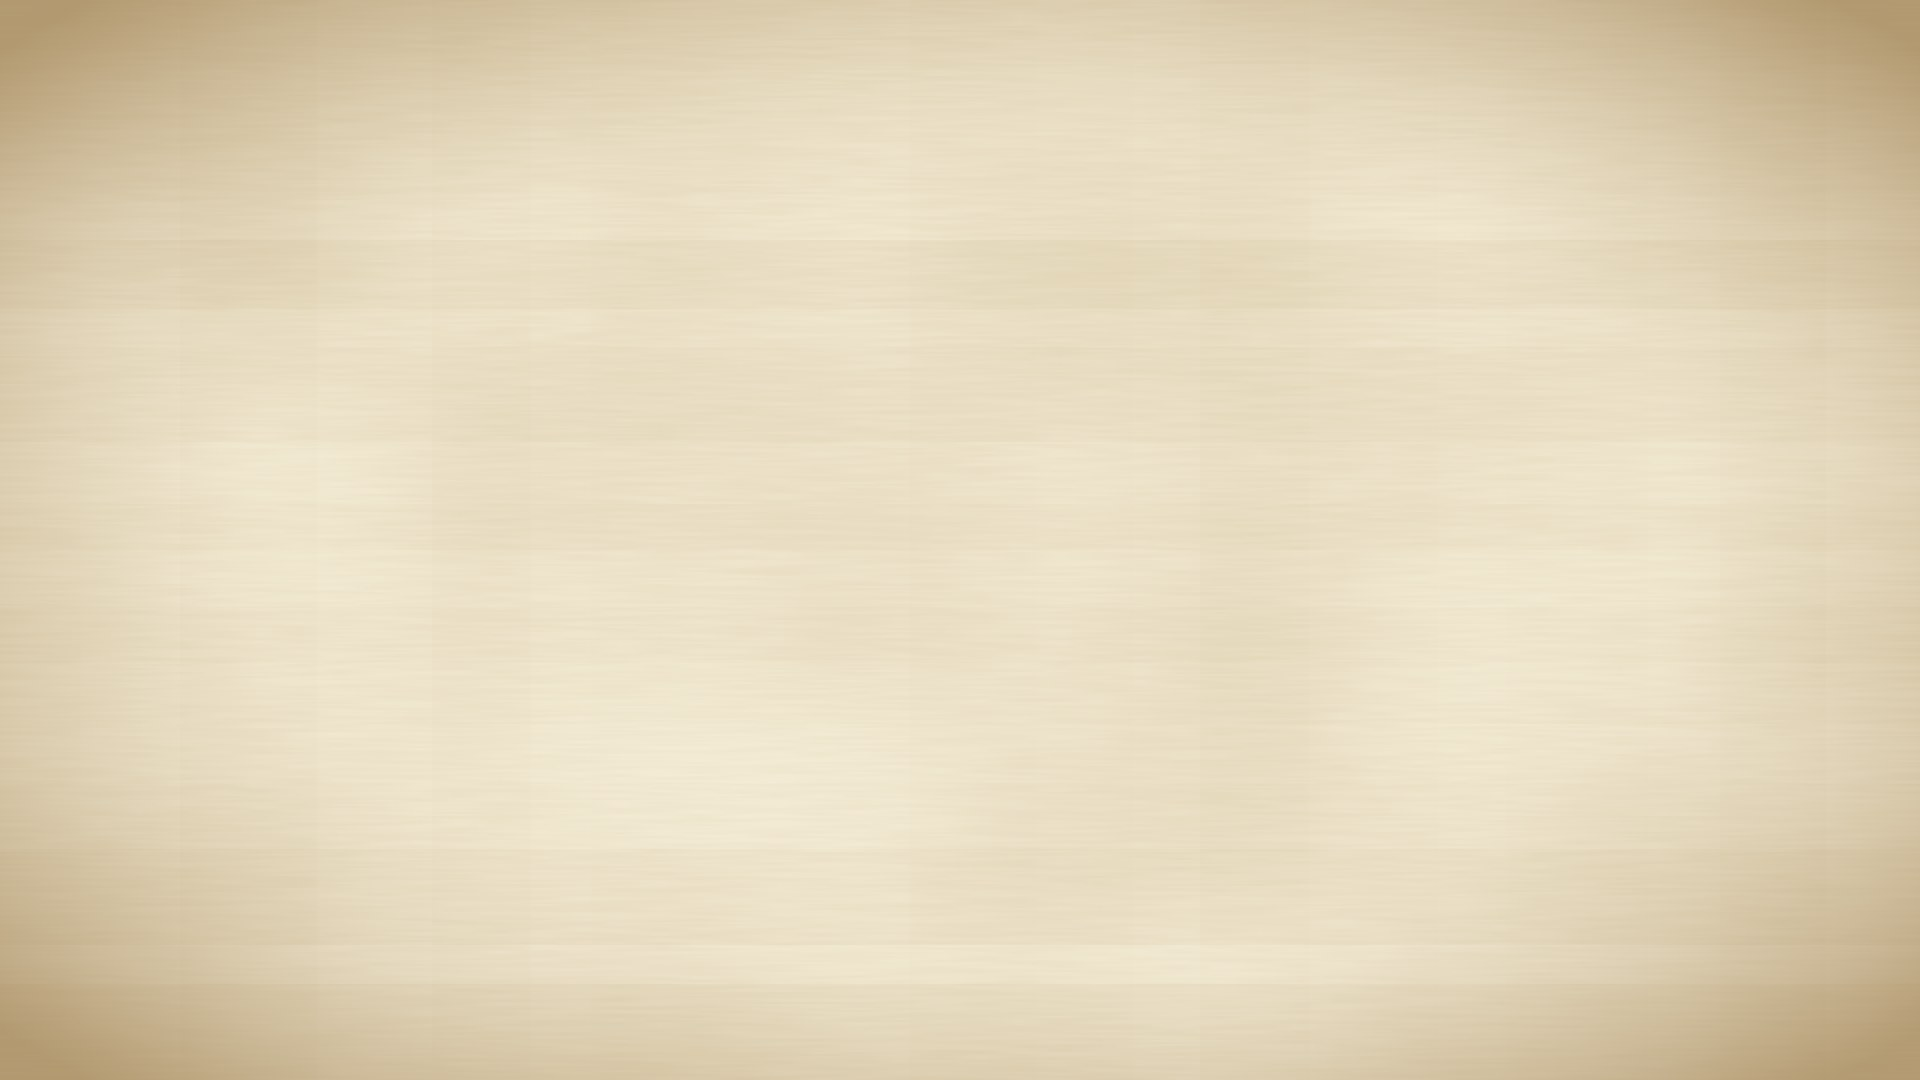
\includegraphics[width=\paperwidth,height=\paperheight]{papiro.jpg}}
\setbeamercolor{normal text}{fg=black!88!azuloscuro}
\setbeamercolor{frametitle}{fg=azul}
\setbeamerfont{frametitle}{series=\bfseries}
\setbeamertemplate{section in toc shaded}{\leavevmode{\color{gris}\inserttocsection}\par}
\setbeamercolor{title}{fg=azul}
\setbeamercolor{subtitle}{fg=gris}
\setbeamercolor{item projected}{bg=azul,fg=papiro}
\setbeamertemplate{itemize item}{\small\textcolor{dorado}{$\blacktriangleright$}}
\setbeamertemplate{navigation symbols}{}
% --- Español + hebreo + griego (XeLaTeX) ---
\usepackage[bidi=default]{babel}
\babelprovide[import,main]{spanish}
\babelprovide[import]{hebrew}
\babelprovide[import]{ancientgreek}
\babelfont[hebrew]{sf}[Path=fonts/, BoldFont=NotoHebrewSans-700.ttf]{NotoHebrewSans-400.ttf}
\babelfont[hebrew]{rm}[Path=fonts/, BoldFont=NotoHebrewSans-700.ttf]{NotoHebrewSans-400.ttf}
\babelfont[ancientgreek]{sf}[Path=fonts/]{GFSPorson.otf}
\babelfont[ancientgreek]{rm}[Path=fonts/]{GFSPorson.otf}
\newcommand{\heb}[1]{\mbox{\foreignlanguage{hebrew}{#1}}}
\newcommand{\grc}[1]{\foreignlanguage{ancientgreek}{#1}}
\newcommand{\SENOR}{S{\fontsize{0.78em}{1em}\selectfont EÑOR}}
% --- Citas (cuadro de un solo color), imágenes, referencias ---
\usepackage[most]{tcolorbox}
\newtcolorbox{cita}[1][]{enhanced, colback=azul!7!papiro, opacityback=0.85, colframe=azul,
  boxrule=0pt, leftrule=2.5pt, arc=0pt, left=6pt, right=6pt, top=4pt, bottom=4pt,
  before skip=4pt, after skip=6pt, fontupper=\small\itshape, #1}
\newcommand{\fuente}[1]{\par\hfill{\upshape\bfseries\footnotesize\textcolor{azul}{#1}}}
\makeatletter
\newcommand{\fotolado}[2]{%
  \begin{tikzpicture}[remember picture,overlay]
    \node[anchor=north east,inner sep=0pt] (foto) at ([xshift=-\beamer@sidebarwidth]current page.north east)
      {\includegraphics[height=\paperheight]{#1}};
    \node[anchor=south east,inner sep=2pt,text=papiro,fill=azuloscuro,fill opacity=0.6,text opacity=1,
      font=\fontsize{4.5}{5.5}\selectfont,align=right,text width=4.2cm] at ([xshift=-3pt,yshift=3pt]foto.south east)
      {\textit{Nota.} #2};
  \end{tikzpicture}}
\makeatother
\newcommand{\refapa}[1]{\par{\RaggedRight\hangindent=1.2em\hangafter=1\noindent #1\par}\vspace{3pt}}
\usepackage{xurl}\urlstyle{same}
\newcommand{\destacar}[1]{\textbf{\textcolor{azul}{#1}}}
\newcommand{\precision}[1]{{\footnotesize\color{gris}\textbf{Precisión:} #1}}
\tikzset{caja/.style={draw=azul,line width=0.8pt,fill=papiro,fill opacity=0.92,text opacity=1,rounded corners=3pt,inner sep=5pt,font=\scriptsize}}
\title[El Dios presente]{\bfseries{El Dios que llena el cielo y la tierra}}
\subtitle{``¿No lleno yo, dice \SENOR, el cielo y la tierra?'' (Jer 23:24)}
\author{}\institute{}\date{}
\titlegraphic{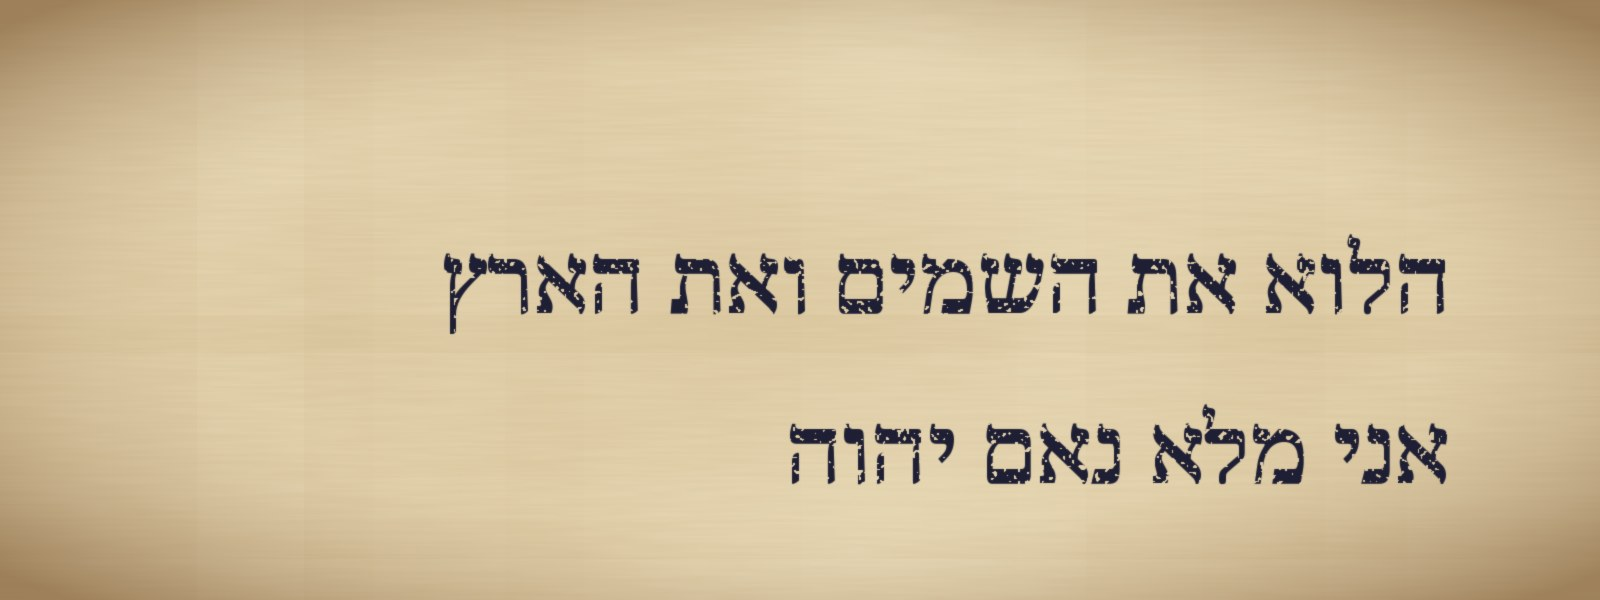
\includegraphics[width=0.80\linewidth,height=0.36\textheight,keepaspectratio]{portada.jpg}\\[-1pt]
  {\fontsize{5}{6}\selectfont\color{gris}\textit{Nota.} Elaboración propia: Jer 23:24b en texto hebreo consonántico (BHS).}}
\begin{document}
\frame{\titlepage}


% ------------------------------------------------------------------
\section{Contexto}

\begin{frame}{``¿Dónde está tu Dios?''}
\begin{columns}[c,onlytextwidth]
\begin{column}{0.50\textwidth}
\begin{cita}Fueron mis lágrimas mi pan de día y de noche, Mientras me dicen todos los días: ¿Dónde está tu Dios?\fuente{(Sal 42:3, RVR1960)}\end{cita}
\begin{cita}Nuestro Dios está en los cielos; Todo lo que quiso ha hecho.\fuente{(Sal 115:3, RVR1960)}\end{cita}
\end{column}
\begin{column}{0.48\textwidth}\small
\begin{itemize}
\item La pregunta atraviesa la Escritura: la hacen los burladores y las naciones.
\item La respuesta tiene dos caras: Dios está \destacar{en los cielos} y está \destacar{aquí}.
\item ``\SENOR{} es Dios arriba en el cielo y abajo en la tierra, y no hay otro'' (Dt 4:39; cf. Jos 2:11).
\end{itemize}
\end{column}
\end{columns}
\end{frame}

\begin{frame}{Un atributo de la Identidad}
\centering
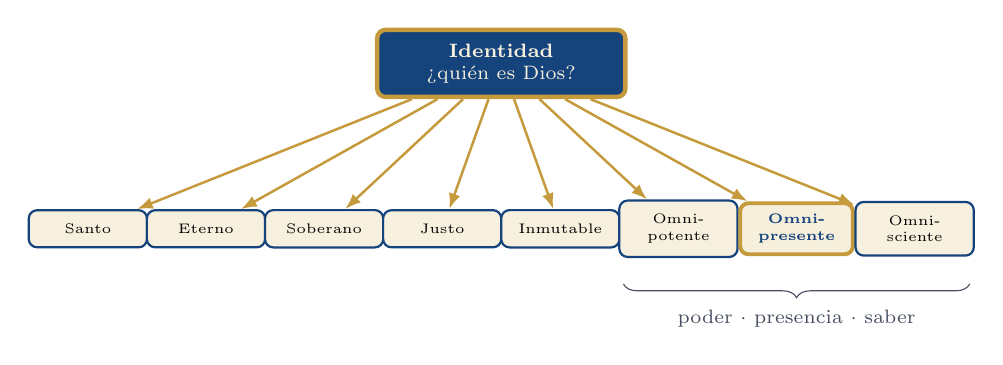
\begin{tikzpicture}[font=\scriptsize]
 \node[draw=dorado,line width=1.6pt,fill=azul,text=papiro,rounded corners=3pt,text width=2.8cm,align=center,inner sep=5pt] (s) at (0,1.9) {\textbf{Identidad}\\ ¿quién es Dios?};
 \foreach \x/\n/\t in {-5.25/a/Santo, -3.75/b/Eterno, -2.25/c/Soberano, -0.75/d/Justo, 0.75/e/Inmutable, 2.25/f/{Omni-\\potente}}{
   \node[caja,text width=1.15cm,align=center,font=\tiny] (\n) at (\x,-0.2) {\t};
   \draw[-{Latex[length=2mm]},dorado,line width=0.9pt](s)--(\n);}
 \node[draw=dorado,line width=1.4pt,fill=papiro,rounded corners=3pt,text width=1.15cm,align=center,inner sep=4pt,font=\tiny] (g) at (3.75,-0.2) {\textbf{\textcolor{azul}{Omni-\\presente}}};
 \node[caja,text width=1.15cm,align=center,font=\tiny] (h) at (5.25,-0.2) {Omni-\\sciente};
 \draw[-{Latex[length=2mm]},dorado,line width=0.9pt](s)--(g); \draw[-{Latex[length=2mm]},dorado,line width=0.9pt](s)--(h);
 \draw[decorate,decoration={brace,amplitude=5pt,mirror},gris] (1.55,-0.9)--(5.95,-0.9) node[midway,below=6pt,text=gris]{poder $\cdot$ presencia $\cdot$ saber};
\end{tikzpicture}\par\medskip
\begin{columns}[t,onlytextwidth]
\begin{column}{0.52\textwidth}\scriptsize
Charnock reúne la tríada: ``Como su esencia es inmensa, no puede ser confinada en un lugar; como es eterno, no puede medirse en el tiempo; así que como es todopoderoso, no puede ser limitado'' (citado en Pink, 2020, cap. 9, p. 47).
\end{column}
\begin{column}{0.46\textwidth}
\precision{clasificación propuesta: Identidad; \emph{incomunicable}. Ninguna criatura está en dos lugares a la vez; lo que se comunica es su presencia: Dios habita en su pueblo (1 Co 3:16).}
\end{column}
\end{columns}
\end{frame}

\begin{frame}{``Omnipresente'': una palabra teológica}
\begin{columns}[c,onlytextwidth]
\begin{column}{0.46\textwidth}\small
\begin{itemize}
\item Del latín \emph{omnipraesens}: \emph{omnis}, ``todo'', y \emph{praesens}, ``presente''.
\item ``Cuando la Biblia afirma que Dios es omnipresente, quiere decir que Él siempre está presente en todo lugar en toda Su plenitud'' (Washer, 2021, p. 89).
\item La palabra no está en la Biblia; la verdad sí, de punta a punta.
\end{itemize}
\end{column}
\begin{column}{0.52\textwidth}
\scriptsize\renewcommand{\arraystretch}{1.15}
\begin{tabular}{@{}>{\RaggedRight\arraybackslash}p{1.7cm}>{\RaggedRight\arraybackslash}p{2.0cm}>{\RaggedRight\arraybackslash}p{2.4cm}@{}}
\toprule
\textbf{RVR1960} & \textbf{Original} & \textbf{Ejemplo} \\ \midrule
``presencia'' AT (182) & \heb{פָּנִים}, \heb{לִפְנֵי} & Éx 33:14 \\
``presencia'' NT (26) & \grc{πρόσωπον}, \grc{ἐνώπιον} & 2 Ts 1:9 \\ \midrule
\textbf{Total} & \textbf{208 veces} & en 204 versículos \\
\bottomrule
\end{tabular}\par\smallskip
\precision{conteo propio con la RVR1960 sin títulos; verificar en e-Sword.}
\end{column}
\end{columns}
\end{frame}

% ------------------------------------------------------------------
\section{Jeremías 23}

\begin{frame}{Profetas que hablaban sin ser enviados}
\begin{columns}[t,onlytextwidth]
\begin{column}{0.52\textwidth}
\begin{cita}[fontupper=\scriptsize\itshape]No escuchéis las palabras de los profetas que os profetizan; os alimentan con vanas esperanzas; hablan visión de su propio corazón, no de la boca de \SENOR. Dicen atrevidamente a los que me irritan: \SENOR{} dijo: Paz tendréis\ldots\fuente{(Jer 23:16--17, RVR1960)}\end{cita}
\begin{cita}[fontupper=\scriptsize\itshape]No envié yo aquellos profetas, pero ellos corrían; yo no les hablé, mas ellos profetizaban.\fuente{(Jer 23:21, RVR1960)}\end{cita}
\end{column}
\begin{column}{0.46\textwidth}\small
\begin{itemize}
\item Jer 23:9--40: oráculo contra los profetas de Jerusalén.
\item ``Aun en mi casa hallé su maldad'' (23:11).
\item Hablaban en nombre de Dios como si Dios estuviera \destacar{lejos}: sin oír y sin ver.
\item A ellos se dirigen tres preguntas.
\end{itemize}
\end{column}
\end{columns}
\end{frame}

\begin{frame}{Texto ancla: Jer 23:23--24}
\fotolado{panel_jeremias23.jpg}{Elaboración propia: Jer 23:24 en texto hebreo consonántico (BHS).}
\begin{columns}[c,onlytextwidth]
\begin{column}{0.58\textwidth}
\begin{cita}¿Soy yo Dios de cerca solamente, dice \SENOR, y no Dios desde muy lejos? ¿Se ocultará alguno, dice \SENOR, en escondrijos que yo no lo vea? ¿No lleno yo, dice \SENOR, el cielo y la tierra?\fuente{(Jer 23:23--24, RVR1960)}\end{cita}
\end{column}
\begin{column}{0.40\textwidth}\end{column}
\end{columns}
\end{frame}

\begin{frame}{Jer 23:23--24 en hebreo}
\begin{center}\scriptsize\heb{הַאֱלֹהֵי מִקָּרֹב אָנִי נְאֻם־יְהוָה וְלֹא אֱלֹהֵי מֵרָחֹק}\\[1pt]\heb{הֲלוֹא אֶת־הַשָּׁמַיִם וְאֶת־הָאָרֶץ אֲנִי מָלֵא נְאֻם־יְהוָה}\end{center}
\scriptsize\renewcommand{\arraystretch}{1.1}
\begin{tabular}{@{}>{\RaggedRight\arraybackslash}p{2.8cm}>{\RaggedRight\arraybackslash}p{0.9cm}>{\RaggedRight\arraybackslash}p{8.1cm}@{}}
\toprule
\heb{הַאֱלֹהֵי מִקָּרֹב} & \heb{קרב} & ``¿Dios de cerca?''. \emph{Qarov}: cercano en espacio y en parentesco (Dt 4:7). ``Solamente'' es un añadido de la RVR1960. \\
\heb{מֵרָחֹק} \emph{merajoq} & \heb{רחק} & ``desde lejos'', en el espacio y en el tiempo (Is 37:26). \\
\heb{יִסָּתֵר בַּמִּסְתָּרִים} & \heb{סתר} & ``¿se esconderá en los escondites?'': la raíz repetida cierra la salida. \\
\heb{אֲנִי מָלֵא} & \heb{מלא} & ``yo lleno'': un estado permanente; el sujeto enfatizado. \\
\heb{נְאֻם־יְהוָה} & \heb{נאם} & ``dice el \SENOR'': tres veces en dos versículos; cada pregunta lleva firma. \\
\bottomrule
\end{tabular}
\end{frame}

\begin{frame}{Tres preguntas}
\centering
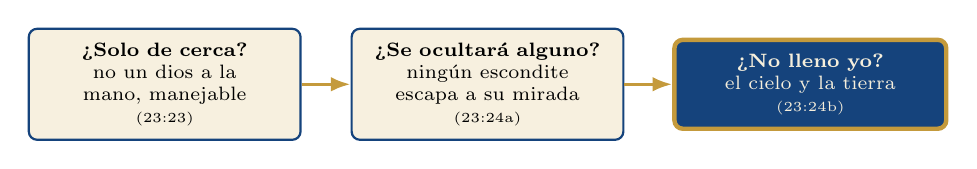
\begin{tikzpicture}[font=\scriptsize]
 \node[caja,text width=3.1cm,align=center] (a) at (0,0) {\textbf{¿Solo de cerca?}\\ no un dios a la mano, manejable\\ {\tiny(23:23)}};
 \node[caja,text width=3.1cm,align=center] (b) at (4.1,0) {\textbf{¿Se ocultará alguno?}\\ ningún escondite escapa a su mirada\\ {\tiny(23:24a)}};
 \node[draw=dorado,line width=1.6pt,fill=azul,text=papiro,rounded corners=3pt,text width=3.1cm,align=center,inner sep=5pt] (c) at (8.2,0) {\textbf{¿No lleno yo?}\\ el cielo y la tierra\\ {\tiny(23:24b)}};
 \draw[-{Latex[length=2.5mm]},dorado,line width=1.2pt] (a)--(b); \draw[-{Latex[length=2.5mm]},dorado,line width=1.2pt] (b)--(c);
\end{tikzpicture}\par\medskip
\begin{columns}[t,onlytextwidth]
\begin{column}{0.52\textwidth}\small
\begin{itemize}
\item Los falsos profetas trataban a Dios como a un dios \destacar{de cerca}: uno que firma lo que el profeta ya decidió.
\item Dios responde: también soy \destacar{de lejos}, el que está sobre todo; y por eso nada queda fuera de mi alcance.
\end{itemize}
\end{column}
\begin{column}{0.46\textwidth}\scriptsize
MacArthur: Dios ``aquí se declara omnipresente y omnisciente, tanto en sentido inmanente como trascendente'' (MacArthur, 2011, nota a Jer 23:23).
\end{column}
\end{columns}
\end{frame}

\begin{frame}{¿Cerca o lejos? Tres lecturas antiguas}
\scriptsize\renewcommand{\arraystretch}{1.18}
\begin{tabular}{@{}>{\RaggedRight\arraybackslash}p{2.0cm}>{\RaggedRight\arraybackslash}p{5.2cm}>{\RaggedRight\arraybackslash}p{4.6cm}@{}}
\toprule
\textbf{Texto} & \textbf{Lectura} & \textbf{Sentido} \\ \midrule
TM & pregunta: ``¿Soy yo Dios de cerca\ldots{} y no Dios desde muy lejos?'' & no solo cercano y manejable: también el lejano, sobre todo \\
LXX & afirmación: \grc{θεὸς ἐγγίζων ἐγώ εἰμι\ldots{} καὶ οὐχὶ θεὸς πόρρωθεν}, ``Dios que se acerca soy yo\ldots{} y no Dios de lejos'' & no ausente: cerca de quien obra en secreto \\
Targum Jonatán & ``Yo soy el Dios que creé el mundo desde el principio\ldots{} el Dios que renovaré el mundo para los justos'' & cerca y lejos leídos en el \destacar{tiempo} \\
\bottomrule
\end{tabular}\par\medskip
\precision{(textual) la LXX convierte la pregunta en afirmación. El TM niega que Dios sea solo cercano (y manejable); la LXX, que sea lejano (y ciego): llegan al mismo punto. Se sigue el TM, como la RVR1960. La lectura del Targum es interpretación judía antigua (Sefaria; traducción propia).}
\end{frame}

\begin{frame}{``¿No lleno yo el cielo y la tierra?''}
\begin{columns}[t,onlytextwidth]
\begin{column}{0.50\textwidth}\small
\begin{itemize}
\item \heb{מָלֵא} \emph{male'}: ``unas 250 veces''. En uso transitivo ``tiene el sentido de `llenar' todos los ámbitos, sin necesariamente `llenar' todos los espacios'' (Vine, 1999).
\item Dios no ocupa el mundo como el agua un vaso, por partes: está en todos sus ámbitos con todo su ser.
\end{itemize}
\begin{cita}[fontupper=\scriptsize\itshape]Santo, santo, santo, \SENOR{} de los ejércitos; toda la tierra está llena de su gloria.\fuente{(Is 6:3, RVR1960)}\end{cita}
\end{column}
\begin{column}{0.48\textwidth}\scriptsize\renewcommand{\arraystretch}{1.15}
\begin{tabular}{@{}>{\RaggedRight\arraybackslash}p{1.4cm}>{\RaggedRight\arraybackslash}p{4.3cm}@{}}
\toprule
TM & \heb{אֲנִי מָלֵא} ``yo lleno'' \\
LXX & \grc{ἐγὼ πληρῶ} \\
Targum & \heb{יְקָרִי מְלֵי}: ``\destacar{mi gloria} llena'' \\
Is 6:3 & \heb{מְלֹא כָל־הָאָרֶץ כְּבוֹדוֹ} \\
\bottomrule
\end{tabular}\par\smallskip
\precision{el Targum pone ``mi gloria'' donde el hebreo dice ``yo'': habla de Dios con reverencia, sin atribuirle extensión física.}
\end{column}
\end{columns}
\end{frame}

% ------------------------------------------------------------------
\section{La palabra}

\begin{frame}{Sin una palabra, con muchas}
\centering
\begin{tikzpicture}[font=\scriptsize]
 \node[draw=dorado,line width=1.6pt,fill=azul,text=papiro,circle,minimum size=1.7cm,align=center] (c) at (0,0) {\textbf{La}\\\textbf{presencia}};
 \node[caja,text width=2.7cm,align=center] (p) at (-4.4,1.3) {\heb{פָּנִים} \emph{panim}\\ rostro {\tiny(Éx 33:14)}};
 \node[caja,text width=2.7cm,align=center] (s) at (0,2.0) {\heb{שָׁם} \emph{sham}\\ allí {\tiny(Sal 139:8)}};
 \node[caja,text width=2.7cm,align=center] (i) at (4.4,1.3) {\heb{עִם} \emph{im}\\ con {\tiny(Gn 28:15)}};
 \node[caja,text width=2.7cm,align=center] (q) at (-4.4,-1.3) {\heb{קָרוֹב} \emph{qarov}\\ cerca {\tiny(Sal 145:18)}};
 \node[caja,text width=2.7cm,align=center] (m) at (0,-2.0) {\heb{מָקוֹם} \emph{maqom}\\ lugar {\tiny(Gn 28:16)}};
 \node[caja,text width=2.7cm,align=center] (l) at (4.4,-1.3) {\heb{מָלֵא} \emph{male'}\\ llenar {\tiny(Jer 23:24)}};
 \foreach \n in {p,s,i,q,m,l}\draw[dorado,line width=1.1pt](c)--(\n);
\end{tikzpicture}\par\medskip
\small\RaggedRight El hebreo no tiene un sustantivo para ``omnipresencia'': dice la presencia con un rostro, un adverbio, una preposición, un adjetivo y un verbo. No por definiciones, sino por relaciones.
\end{frame}

\begin{frame}{\emph{Panim}: el rostro que acompaña}
\begin{columns}[c,onlytextwidth]
\begin{column}{0.50\textwidth}
\begin{cita}Y él dijo: Mi presencia irá contigo, y te daré descanso. Y Moisés respondió: Si tu presencia no ha de ir conmigo, no nos saques de aquí.\fuente{(Éx 33:14--15, RVR1960)}\end{cita}
\begin{center}\heb{פָּנַי יֵלֵכוּ וַהֲנִחֹתִי לָךְ}\end{center}
\end{column}
\begin{column}{0.48\textwidth}\small
\begin{itemize}
\item \heb{פָּנִים}: ``rostro, faz''; ``unas 2.100 veces'', siempre en plural (Vine, 1999).
\item Literalmente: ``\destacar{Mi rostro} irá''. Moisés no pide un lugar: pide una compañía.
\item \heb{לִפְנֵי יְהוָה}, ``delante del \SENOR'': la forma más frecuente de la presencia.
\item \heb{לֶחֶם הַפָּנִים}, ``pan del rostro'' (RVR1960: ``de la proposición'', Nm 4:7).
\end{itemize}
\end{column}
\end{columns}
\end{frame}

\begin{frame}{\emph{Sham}: ``allí estás tú''}
\fotolado{panel_salmo139.jpg}{Elaboración propia: Sal 139:7--8 en texto hebreo consonántico (BHS).}
\begin{columns}[c,onlytextwidth]
\begin{column}{0.58\textwidth}
\begin{cita}[fontupper=\scriptsize\itshape]¿A dónde me iré de tu Espíritu? ¿Y a dónde huiré de tu presencia? Si subiere a los cielos, allí estás tú; Y si en el Seol hiciere mi estrado, he aquí, allí tú estás. Si tomare las alas del alba Y habitare en el extremo del mar, Aun allí me guiará tu mano, Y me asirá tu diestra. Si dijere: Ciertamente las tinieblas me encubrirán; Aun la noche resplandecerá alrededor de mí. Aun las tinieblas no encubren de ti, Y la noche resplandece como el día; Lo mismo te son las tinieblas que la luz.\fuente{(Sal 139:7--12, RVR1960)}\end{cita}
\end{column}
\begin{column}{0.40\textwidth}\end{column}
\end{columns}
\end{frame}

\begin{frame}{Sal 139:7--12: filología}
\begin{center}\heb{אִם־אֶסַּק שָׁמַיִם שָׁם אָתָּה וְאַצִּיעָה שְׁאוֹל הִנֶּךָּ}\end{center}
\scriptsize\renewcommand{\arraystretch}{1.1}
\begin{tabular}{@{}>{\RaggedRight\arraybackslash}p{2.7cm}>{\RaggedRight\arraybackslash}p{9.1cm}@{}}
\toprule
\heb{מֵרוּחֶךָ} // \heb{מִפָּנֶיךָ} & ``de tu Espíritu'' // ``de tu rostro'': el Espíritu de Dios es Dios presente. \\
\heb{אֶבְרָח} \emph{evraj} & ``huiré'': el mismo verbo de Jonás, ``para huir'' (\heb{לִבְרֹחַ}) de delante del \SENOR{} (Jon 1:3). \\
\heb{שָׁם אָתָּה} & ``allí tú'', sin verbo: la presencia se afirma sin decir ``estás''. \\
\heb{הִנֶּךָּ} & ``¡he aquí tú!'': exclamación de hallazgo, en el Seol mismo. \\
\heb{כַנְפֵי־שָׁחַר} & ``alas del alba'' (oriente) y ``extremo del mar'' (occidente). \\
LXX 138:8 & \grc{ἐὰν καταβῶ εἰς τὸν ᾅδην, πάρει}: ``si bajo al Hades, \destacar{estás presente}'' (\grc{πάρειμι}). \\
\bottomrule
\end{tabular}\par\smallskip
\precision{el Sal 139 es el texto ancla de \emph{Omnisciente}; aquí se lee solo la estrofa de la presencia (vv. 7--12). Dios conoce porque está, y está para conocer.}
\end{frame}

\begin{frame}{Consuelo y advertencia}
\centering
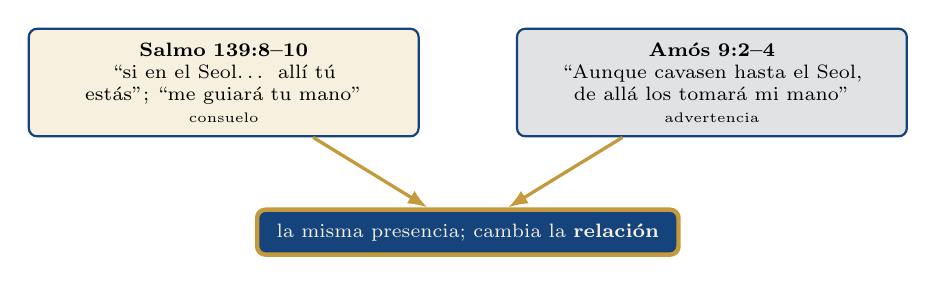
\begin{tikzpicture}[font=\scriptsize]
 \node[caja,text width=4.6cm,align=center] (a) at (0,0) {\textbf{Salmo 139:8--10}\\ ``si en el Seol\ldots{} allí tú estás''; ``me guiará tu mano''\\ {\tiny consuelo}};
 \node[caja,text width=4.6cm,align=center,fill=gris!18] (b) at (6.2,0) {\textbf{Amós 9:2--4}\\ ``Aunque cavasen hasta el Seol, de allá los tomará mi mano''\\ {\tiny advertencia}};
 \node[draw=dorado,line width=1.6pt,fill=azul,text=papiro,rounded corners=3pt,text width=5.0cm,align=center,inner sep=5pt] (c) at (3.1,-1.9) {la misma presencia; cambia la \textbf{relación}};
 \draw[-{Latex[length=2.5mm]},dorado,line width=1.2pt](a)--(c); \draw[-{Latex[length=2.5mm]},dorado,line width=1.2pt](b)--(c);
\end{tikzpicture}\par\medskip
\small\RaggedRight Amós repite cinco veces \heb{מִשָּׁם}, ``de allí'' (9:2--4): cielo, Seol, Carmelo, fondo del mar, cautiverio. No hay escondite.
\end{frame}

\begin{frame}{\emph{Im} y \emph{qarov}: ``contigo'' y ``cerca''}
\begin{columns}[t,onlytextwidth]
\begin{column}{0.50\textwidth}
\begin{cita}[fontupper=\scriptsize\itshape]Porque ¿qué nación grande hay que tenga dioses tan cercanos a ellos como lo está \SENOR{} nuestro Dios en todo cuanto le pedimos?\fuente{(Dt 4:7, RVR1960)}\end{cita}
\begin{cita}[fontupper=\scriptsize\itshape]Cercano está \SENOR{} a todos los que le invocan, A todos los que le invocan de veras.\fuente{(Sal 145:18, RVR1960)}\end{cita}
\end{column}
\begin{column}{0.48\textwidth}\small
\begin{itemize}
\item \heb{עִם}: ``He aquí, yo estoy contigo'' (\heb{אָנֹכִי עִמָּךְ}, Gn 28:15); ``yo estaré contigo'' (Is 43:2).
\item De aquí sale \heb{עִמָּנוּאֵל}, ``con nosotros, Dios''.
\item \heb{קָרוֹב}: la cercanía bíblica es la de quien \destacar{oye}.
\item Las naciones tenían dioses visibles; Israel, un Dios sin imagen y más cercano.
\end{itemize}
\end{column}
\end{columns}
\end{frame}

\begin{frame}{\emph{Maqom} y \emph{kul}: el lugar que no lo contiene}
\begin{columns}[c,onlytextwidth]
\begin{column}{0.50\textwidth}
\begin{cita}Pero ¿es verdad que Dios morará sobre la tierra? He aquí que los cielos, los cielos de los cielos, no te pueden contener; ¿cuánto menos esta casa que yo he edificado?\fuente{(1 R 8:27, RVR1960)}\end{cita}
\begin{center}\scriptsize\heb{הִנֵּה הַשָּׁמַיִם וּשְׁמֵי הַשָּׁמַיִם לֹא יְכַלְכְּלוּךָ}\end{center}
\end{column}
\begin{column}{0.48\textwidth}\small
\begin{itemize}
\item \heb{כּוּל} \emph{kul}, forma intensiva: ``contener, abarcar''.
\item ``Los cielos de los cielos'': superlativo, lo más alto pensable.
\item \heb{מָקוֹם}: ``los ojos de \SENOR{} están en \destacar{todo lugar}'' (\heb{בְּכָל־מָקוֹם}, Pr 15:3).
\item Pero Salomón pide que Dios oiga ``en este lugar'' (8:30): ninguna casa lo contiene, y él se compromete a escuchar allí.
\end{itemize}
\end{column}
\end{columns}
\end{frame}

\begin{frame}{El espectro completo}
\scriptsize\renewcommand{\arraystretch}{1.1}
\begin{tabular}{@{}>{\RaggedRight\arraybackslash}p{2.4cm}>{\RaggedRight\arraybackslash}p{2.6cm}>{\RaggedRight\arraybackslash}p{3.0cm}>{\RaggedRight\arraybackslash}p{3.8cm}@{}}
\toprule
\textbf{Término} & \textbf{Sentido} & \textbf{LXX / NT} & \textbf{Textos} \\ \midrule
\heb{פָּנִים} \emph{panim} & rostro, presencia & \grc{πρόσωπον} & Éx 33:14; Jon 1:3; 2 Ts 1:9 \\
\heb{שָׁם} \emph{sham} & allí & \grc{ἐκεῖ} & Sal 139:8; Am 9:2; Ez 48:35 \\
\heb{עִם} \emph{im} & con & \grc{μετά} & Gn 28:15; Is 7:14; Mt 28:20 \\
\heb{קָרוֹב} \emph{qarov} & cercano & \grc{ἐγγύς} & Dt 4:7; Sal 145:18; Flp 4:5 \\
\heb{מָקוֹם} \emph{maqom} & lugar & \grc{τόπος} & Gn 28:16; Pr 15:3 \\
\heb{מָלֵא} \emph{male'} & llenar & \grc{πληρόω} & Is 6:3; Jer 23:24; Ef 4:10 \\
\heb{כּוּל} \emph{kul} & contener & \grc{ἀρκέω} & 1 R 8:27; 2 Cr 2:6 \\
--- & estar presente & \grc{πάρειμι} & Sal 138:8 LXX \\
\heb{שָׁכַן} \emph{shajan} & habitar & \grc{σκηνόω}, \grc{ἐνοικέω} & Éx 25:8; Jn 1:14; 2 Co 6:16 \\
\bottomrule
\end{tabular}\par\smallskip
\precision{elaboración propia a partir de Vine (1999), la BHS, Rahlfs-Hanhart (2006) y NA28.}
\end{frame}

\begin{frame}{Del hebreo a Pablo}
\centering
\begin{tikzpicture}[font=\scriptsize]
 \node[caja,text width=3.2cm,align=center] (a1) at (0,1.3) {\textbf{Hebreo}\\ \heb{אֲנִי מָלֵא} ``yo lleno''\\ {\tiny(Jer 23:24)}};
 \node[caja,text width=3.2cm,align=center] (b1) at (4.2,1.3) {\textbf{LXX}\\ \grc{ἐγὼ πληρῶ}\\ {\tiny(Jer 23:24)}};
 \node[draw=dorado,line width=1.4pt,fill=azul,text=papiro,rounded corners=3pt,text width=3.2cm,align=center,inner sep=5pt] (c1) at (8.4,1.3) {\textbf{Pablo}\\ \grc{ἵνα πληρώσῃ τὰ πάντα}\\ {\tiny(Ef 4:10)}};
 \node[caja,text width=3.2cm,align=center] (a2) at (0,-0.9) {\textbf{Hebreo}\\ \heb{קָרוֹב יְהוָה}\\ {\tiny(Sal 145:18)}};
 \node[caja,text width=3.2cm,align=center] (b2) at (4.2,-0.9) {\textbf{LXX}\\ \grc{ἐγγὺς κύριος}\\ {\tiny(Sal 144:18)}};
 \node[draw=dorado,line width=1.4pt,fill=azul,text=papiro,rounded corners=3pt,text width=3.2cm,align=center,inner sep=5pt] (c2) at (8.4,-0.9) {\textbf{Pablo}\\ \grc{ὁ κύριος ἐγγύς}\\ {\tiny(Flp 4:5)}};
 \draw[-{Latex[length=2.5mm]},dorado,line width=1.2pt] (a1)--(b1); \draw[-{Latex[length=2.5mm]},dorado,line width=1.2pt] (b1)--(c1);
 \draw[-{Latex[length=2.5mm]},dorado,line width=1.2pt] (a2)--(b2); \draw[-{Latex[length=2.5mm]},dorado,line width=1.2pt] (b2)--(c2);
\end{tikzpicture}\par\medskip
{\small\itshape\color{gris}Lo que en Jeremías dice el \SENOR{} de sí mismo, en Efesios se dice de Cristo; la cercanía del salmo es la de Filipenses.}
\end{frame}

% ------------------------------------------------------------------
\section{El Nombre}

\begin{frame}{\SENOR-sama: ``el \SENOR{} está allí''}
\fotolado{panel_ezequiel48.jpg}{Elaboración propia: Ez 48:35b en texto hebreo consonántico (BHS).}
\begin{columns}[c,onlytextwidth]
\begin{column}{0.58\textwidth}
\begin{cita}En derredor tendrá dieciocho mil cañas. Y el nombre de la ciudad desde aquel día será \SENOR-sama.\fuente{(Ez 48:35, RVR1960)}\end{cita}
\small
\begin{itemize}
\item La gloria se fue del templo (Ez 10:18; 11:23) y volvió: ``la gloria de \SENOR{} llenó la casa'' (43:5).
\item El libro termina con un nombre: la ciudad se define por quien la habita.
\end{itemize}
\end{column}
\begin{column}{0.40\textwidth}\end{column}
\end{columns}
\end{frame}

\begin{frame}{Ez 48:35: filología}
\begin{center}\heb{וְשֵׁם־הָעִיר מִיּוֹם יְהוָה שָׁמָּה}\end{center}
\scriptsize\renewcommand{\arraystretch}{1.12}
\begin{tabular}{@{}>{\RaggedRight\arraybackslash}p{2.8cm}>{\RaggedRight\arraybackslash}p{9.0cm}@{}}
\toprule
\heb{וְשֵׁם־הָעִיר} & ``y el nombre de la ciudad'': Jerusalén ni se nombra. \\
\heb{מִיּוֹם} & ``desde (aquel) día'': un nombre que ya no cambia. \\
\heb{יְהוָה שָׁמָּה} & ``el \SENOR{} (está) allí''; juego de sonido entre \heb{שֵׁם} (\emph{shem}, ``nombre'') y \heb{שָׁמָּה} (\emph{shammá}, ``allí''). \\
Targum Jonatán & \heb{מִיוֹמָא דִי יִשְׁרֵי יְיָ שְׁכִנְתֵּיהּ תַּמָן}: ``desde el día en que el \SENOR{} haga reposar su \destacar{Shejiná} allí''. \\
\bottomrule
\end{tabular}\par\medskip
\begin{columns}[t,onlytextwidth]
\begin{column}{0.52\textwidth}\scriptsize
MacArthur: ``la consumación de la historia de Israel: ¡el regreso de la presencia de Dios!'' (MacArthur, 2011, nota a Ez 48:35).
\end{column}
\begin{column}{0.46\textwidth}
\precision{(textual) la LXX no traduce el nombre: parece leer \heb{שמה} como \emph{shemáh}, ``su nombre''. Se sigue el TM.}
\end{column}
\end{columns}
\end{frame}

\begin{frame}{Emanuel: ``Dios con nosotros''}
\begin{columns}[t,onlytextwidth]
\begin{column}{0.50\textwidth}
\begin{cita}[fontupper=\scriptsize\itshape]Por tanto, el Señor mismo os dará señal: He aquí que la virgen concebirá, y dará a luz un hijo, y llamará su nombre Emanuel.\fuente{(Is 7:14, RVR1960)}\end{cita}
\begin{cita}[fontupper=\scriptsize\itshape]He aquí, una virgen concebirá y dará a luz un hijo, Y llamarás su nombre Emanuel, que traducido es: Dios con nosotros.\fuente{(Mt 1:23, RVR1960)}\end{cita}
\end{column}
\begin{column}{0.48\textwidth}\small
\begin{itemize}
\item \heb{עִמָּנוּ אֵל}: ``con nosotros, Dios''; grito de confianza ante Asiria: ``porque Dios está con nosotros'' (Is 8:10).
\item Mateo: \grc{μεθ’ ἡμῶν ὁ θεός}.
\item La presencia tiene ahora rostro humano.
\end{itemize}
\precision{la señal se dio a Acaz (7:16); \heb{עַלְמָה} es ``joven''; la LXX tradujo \grc{παρθένος}, y Mateo cita la LXX. La serie sigue la lectura cristiana del cumplimiento pleno en Jesús.}
\end{column}
\end{columns}
\end{frame}

\begin{frame}{Nombres y declaraciones de la presencia}
\scriptsize\renewcommand{\arraystretch}{1.12}
\begin{tabular}{@{}>{\RaggedRight\arraybackslash}p{4.4cm}>{\RaggedRight\arraybackslash}p{4.6cm}>{\RaggedRight\arraybackslash}p{2.7cm}@{}}
\toprule
\textbf{Nombre o declaración} & \textbf{Original} & \textbf{Texto} \\ \midrule
\SENOR-sama & \heb{יְהוָה שָׁמָּה} & Ez 48:35 \\
Emanuel & \heb{עִמָּנוּאֵל}; \grc{μεθ’ ἡμῶν ὁ θεός} & Is 7:14; Mt 1:23 \\
Dios de cerca y de lejos & \heb{אֱלֹהֵי מִקָּרֹב}\ldots{} \heb{מֵרָחֹק} & Jer 23:23 \\
Arriba en el cielo y abajo en la tierra & \heb{בַּשָּׁמַיִם מִמַּעַל וְעַל־הָאָרֶץ מִתָּחַת} & Dt 4:39; Jos 2:11 \\
En la altura y con el humilde & \heb{מָרוֹם וְקָדוֹשׁ אֶשְׁכּוֹן וְאֶת־דַּכָּא} & Is 57:15 \\
El Dios de Bet-el & \heb{הָאֵל בֵּית־אֵל} & Gn 31:13 \\
``El Señor está cerca'' & \grc{ὁ κύριος ἐγγύς} & Flp 4:5 \\
\emph{HaMaqom} (rabínico) & \heb{הַמָּקוֹם} & Bereshit Rabá 68:9 \\
\bottomrule
\end{tabular}\par\smallskip
\precision{el Nombre del atributo en esta serie es \SENOR-sama, y su cumplimiento personal, Emanuel. Es un nombre de lugar: no ``Dios está en todas partes'', sino ``Dios está \destacar{allí}'', con su pueblo.}
\end{frame}

% ------------------------------------------------------------------
\section{Definición}

\begin{frame}{¿Qué es la omnipresencia?}
\begin{columns}[c,onlytextwidth]
\begin{column}{0.48\textwidth}
\begin{tcolorbox}[colback=papiro,colframe=azul,boxrule=1pt,arc=3pt,title={\small Definición},colbacktitle=azul,coltitle=papiro]
\small La omnipresencia es la perfección eterna de Dios por la cual él, sin ser contenido por ningún lugar, está presente con \destacar{todo su ser} en todo lugar: llena el cielo y la tierra, sostiene y ve todas las cosas, y se hace presente de manera especial para habitar con su pueblo, para juzgar al pecador y, en plenitud, en el \destacar{Hijo}.
\end{tcolorbox}
\precision{definición de síntesis de esta serie.}
\end{column}
\begin{column}{0.50\textwidth}
\scriptsize\renewcommand{\arraystretch}{1.12}
\begin{tabular}{@{}>{\RaggedRight\arraybackslash}p{1.9cm}>{\RaggedRight\arraybackslash}p{4.3cm}@{}}
\toprule
\textbf{Rasgo} & \textbf{Texto} \\ \midrule
No contenido & ``no te pueden contener'' (1 R 8:27) \\
En todo lugar & ``¿No lleno yo\ldots?'' (Jer 23:24) \\
Con todo su ser & ``allí estás tú'' (Sal 139:8) \\
Que sostiene & ``en él vivimos'' (Hch 17:28) \\
Que ve & ``en todo lugar'' (Pr 15:3) \\
Alto y cercano & ``con el quebrantado'' (Is 57:15) \\
Que se compromete & ``yo estoy contigo'' (Gn 28:15) \\
\bottomrule
\end{tabular}
\end{column}
\end{columns}
\end{frame}

\begin{frame}{Inmensidad y omnipresencia}
\centering
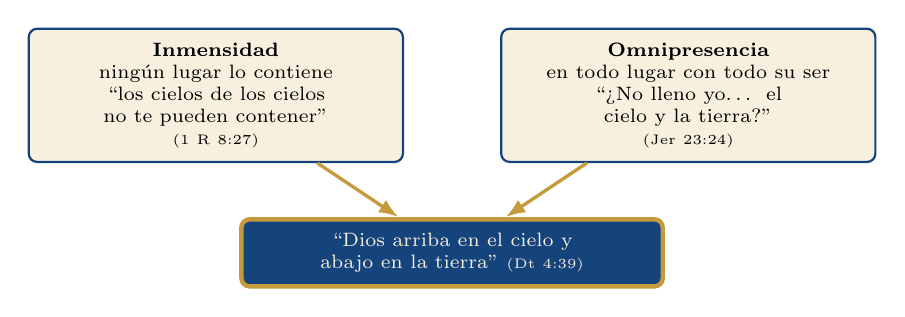
\begin{tikzpicture}[font=\scriptsize]
 \node[caja,text width=4.4cm,align=center] (i) at (0,0) {\textbf{Inmensidad}\\ ningún lugar lo contiene\\ ``los cielos de los cielos no te pueden contener''\\ {\tiny(1 R 8:27)}};
 \node[caja,text width=4.4cm,align=center] (o) at (6.0,0) {\textbf{Omnipresencia}\\ en todo lugar con todo su ser\\ ``¿No lleno yo\ldots{} el cielo y la tierra?''\\ {\tiny(Jer 23:24)}};
 \node[draw=dorado,line width=1.6pt,fill=azul,text=papiro,rounded corners=3pt,text width=5.0cm,align=center,inner sep=5pt] (s) at (3.0,-2.0) {``Dios arriba en el cielo y abajo en la tierra'' {\tiny(Dt 4:39)}};
 \draw[-{Latex[length=2.5mm]},dorado,line width=1.2pt](i)--(s); \draw[-{Latex[length=2.5mm]},dorado,line width=1.2pt](o)--(s);
\end{tikzpicture}\par\medskip
\small\RaggedRight Berkhof: Dios trasciende toda limitación espacial y, sin embargo, está presente en cada punto del espacio con todo su ser (Berkhof, 1938). Sin inmensidad, Dios sería parte del mundo; sin omnipresencia, sería ajeno a él.
\end{frame}

\begin{frame}{Una presencia, varios modos}
\scriptsize\renewcommand{\arraystretch}{1.15}
\begin{tabular}{@{}>{\RaggedRight\arraybackslash}p{2.2cm}>{\RaggedRight\arraybackslash}p{5.4cm}>{\RaggedRight\arraybackslash}p{4.2cm}@{}}
\toprule
\textbf{Modo} & \textbf{Qué hace Dios} & \textbf{Textos} \\ \midrule
Sustentadora & da y mantiene la existencia de todo & Neh 9:6; Hch 17:28; Col 1:17 \\
Que ve y juzga & mira a malos y buenos; nadie escapa & Pr 15:3; Am 9:2--4; He 4:13 \\
De pacto & habita en medio de Israel & Éx 25:8; 29:45; Lv 26:11--12 \\
De gracia & habita en el creyente y en la iglesia & Jn 14:23; 1 Co 3:16; Ef 2:22 \\
Encarnada & ``habitó entre nosotros'' & Jn 1:14; Col 2:9 \\
Gloriosa & ``el tabernáculo de Dios con los hombres'' & Ap 21:3; 22:4 \\
\bottomrule
\end{tabular}\par\medskip
\precision{Dios no está ``más'' en un lugar que en otro en cuanto a su ser; varía la manifestación y la relación. La clasificación es una síntesis teológica, no una lista bíblica.}
\end{frame}

\begin{frame}{Lo que no significa}
\scriptsize\renewcommand{\arraystretch}{1.15}
\begin{tabular}{@{}>{\RaggedRight\arraybackslash}p{3.0cm}>{\RaggedRight\arraybackslash}p{8.8cm}@{}}
\toprule
\textbf{Malentendido} & \textbf{Respuesta bíblica} \\ \midrule
``Dios es todo'' & Llena el mundo, pero no es el mundo: ``Mi mano hizo todas estas cosas'' (Is 66:1--2). \\
Un pedazo en cada lugar & ``La omnipresencia no significa que una parte de Dios está en China y otra parte está en Inglaterra'' (Washer, 2021, p. 89). \\
Una sustancia extendida & ``Precisamente porque es `espíritu', llena el cielo y la tierra'' (Pink, 2020, cap. 16, p. 83). \\
Indiferencia moral & ``vuestras iniquidades han hecho división entre vosotros y vuestro Dios'' (Is 59:2). \\
Todos gozan de su presencia & Hay una presencia que juzga: ``excluidos de la presencia del Señor'' (2 Ts 1:9). \\
Los lugares no importan & Dios eligió lugares de encuentro (Gn 28:17; 1 R 8:29--30); en Cristo, el lugar es una persona (Jn 2:21). \\
\bottomrule
\end{tabular}
\end{frame}

\begin{frame}{Alto y sublime, y con el humilde}
\begin{columns}[c,onlytextwidth]
\begin{column}{0.52\textwidth}
\begin{cita}[fontupper=\scriptsize\itshape]Porque así dijo el Alto y Sublime, el que habita la eternidad, y cuyo nombre es el Santo: Yo habito en la altura y la santidad, y con el quebrantado y humilde de espíritu, para hacer vivir el espíritu de los humildes, y para vivificar el corazón de los quebrantados.\fuente{(Is 57:15, RVR1960)}\end{cita}
\end{column}
\begin{column}{0.46\textwidth}\small
\begin{itemize}
\item \heb{שָׁכַן} \emph{shajan}, ``habitar'', sirve para la altura y para el corazón quebrantado.
\item Es el verbo del tabernáculo (\heb{מִשְׁכָּן}) y de la \emph{Shejiná} (\heb{שְׁכִינָה}).
\item ``¿Quién como \SENOR{} nuestro Dios, que se sienta en las alturas, que se humilla a mirar en el cielo y en la tierra?'' (Sal 113:5--6).
\end{itemize}
\end{column}
\end{columns}
\end{frame}

% ------------------------------------------------------------------
\section{Teología}

\begin{frame}{Presente porque es Espíritu}
\begin{columns}[c,onlytextwidth]
\begin{column}{0.50\textwidth}
\begin{cita}[fontupper=\scriptsize\itshape]Dios es Espíritu; y los que le adoran, en espíritu y en verdad es necesario que adoren.\fuente{(Jn 4:24, RVR1960)}\end{cita}
\scriptsize La samaritana pregunta por lugares (Gerizim o Jerusalén); Jesús responde con el ser de Dios. Un cuerpo ocupa un lugar y deja los demás; Dios, que no tiene cuerpo, no ocupa lugares: \destacar{los llena}. Por eso ``tu Espíritu'' y ``tu presencia'' son paralelos (Sal 139:7).
\end{column}
\begin{column}{0.48\textwidth}\scriptsize
Como observa Pink (2020, cap. 16, p. 83), ``precisamente porque es `espíritu', llena el cielo y la tierra''.\par\medskip
\textbf{Agustín}, \emph{Confesiones} I, 3, 3: ``¿Te contienen, pues, el cielo y la tierra, porque tú los llenas? ¿O los llenas, y sobra algo de ti, porque no te contienen?''\par\smallskip
Es la pregunta de Salomón: ``los cielos de los cielos, no te pueden contener'' (1 R 8:27).\par\smallskip
\precision{traducción propia del latín.}
\end{column}
\end{columns}
\end{frame}

\begin{frame}{Inmenso, eterno y todopoderoso}
\begin{columns}[c,onlytextwidth]
\begin{column}{0.50\textwidth}\scriptsize
La presencia no es una perfección aislada. Charnock une las tres medidas de la criatura: ``Como su esencia es inmensa, no puede ser confinada en un lugar; como es eterno, no puede medirse en el tiempo; así que como es todopoderoso, no puede ser limitado'' (citado en Pink, 2020, cap. 9, p. 47).\par\medskip
\textbf{Berkhof} (1938) lo precisa: \destacar{inmensidad}, Dios sobre el espacio; \destacar{omnipresencia}, Dios en cada punto del espacio con todo su ser.
\end{column}
\begin{column}{0.48\textwidth}
\begin{cita}[fontupper=\scriptsize\itshape]¿No está Dios en la altura de los cielos? Mira lo encumbrado de las estrellas, cuán elevadas están.\fuente{(Job 22:12, RVR1960)}\end{cita}
\precision{Elifaz atribuye a Job la idea de que la altura aleja a Dios: ``Las nubes le rodearon, y no ve'' (Job 22:14). Jeremías responde: Dios es ``de cerca'' y ``desde muy lejos'' a la vez (Jer 23:23).}
\end{column}
\end{columns}
\end{frame}

\begin{frame}{La presencia del Rey}
\begin{columns}[c,onlytextwidth]
\begin{column}{0.50\textwidth}
\begin{cita}[fontupper=\scriptsize\itshape]\SENOR{} estableció en los cielos su trono, y su reino domina sobre todos.\fuente{(Sal 103:19, RVR1960)}\end{cita}
\scriptsize ``El cielo es mi trono, y la tierra estrado de mis pies'' (Is 66:1): el texto que niega que una casa contenga a Dios hace del universo la sala de su trono. \destacar{Llenar es gobernar.}
\end{column}
\begin{column}{0.48\textwidth}\scriptsize
Spurgeon lo advirtió: ``Los hombres permitirán que Dios esté en todas partes, excepto en su Trono'' (citado en Pink, 2020, cap. 6, p. 30).\par\medskip
Muchos aceptan un Dios presente en todas partes siempre que no mande en ninguna. Una omnipresencia sin trono es solo un ambiente; la bíblica es la del Señor que está en todo lugar porque todo lugar le pertenece.
\end{column}
\end{columns}
\end{frame}

\begin{frame}{La presencia que ve}
\begin{columns}[t,onlytextwidth]
\begin{column}{0.50\textwidth}\scriptsize
``¿Se ocultará alguno\ldots{} en escondrijos que yo no lo vea?'' (Jer 23:24). ``Los ojos de \SENOR{} están en todo lugar, mirando a los malos y a los buenos'' (Pr 15:3). Dios conoce porque está, y está para conocer.\par\medskip
De allí un freno moral: ``¡Qué freno sería para nosotros si meditáramos en ello con más frecuencia!'' (Pink, 2020, cap. 3, p. 19).
\end{column}
\begin{column}{0.48\textwidth}\scriptsize
Y una doble consecuencia (Washer, 2021, p. 89): ``Para el cristiano, la omnipresencia de Dios infunde gran confianza y consuelo\ldots{} Para el incrédulo\ldots{} terror porque no hay ninguna posibilidad de esconderse''.\par\medskip
El Salmo 139 las une: ``¿a dónde huiré de tu presencia?'' (v.~7) y ``aun allí me guiará tu mano'' (v.~10). La presencia que impide la fuga es la que sostiene.
\end{column}
\end{columns}
\end{frame}

\begin{frame}{Preguntas que plantea la Escritura}
\scriptsize\renewcommand{\arraystretch}{1.2}
\begin{tabular}{@{}>{\RaggedRight\arraybackslash}p{3.4cm}>{\RaggedRight\arraybackslash}p{8.4cm}@{}}
\toprule
\textbf{Pregunta} & \textbf{Respuesta} \\ \midrule
¿Por qué ``Padre nuestro que estás en los cielos''? & El cielo es el lugar del trono. Salomón pide que Dios oiga ``en los cielos'' (1 R 8:30) y confiesa que los cielos no lo contienen (8:27). ``Dios está en el cielo, y tú sobre la tierra; por tanto, sean pocas tus palabras'' (Ec 5:2). \\
¿Está Dios en el Seol? & ``Si en el Seol hiciere mi estrado\ldots{} allí tú estás'' (Sal 139:8); y, sin embargo, ``excluidos de la presencia del Señor'' (2 Ts 1:9). Presente con su ser y su juicio; ausente su favor. El pecado ``ha hecho ocultar de vosotros su rostro'' (Is 59:2). \\
Si está en todas partes, ¿por qué buscarlo? & La omnipresencia no es comunión: ``me buscaréis y me hallaréis'' (Jer 29:13); ``Acercaos a Dios, y él se acercará a vosotros'' (Stg 4:8). \\
\bottomrule
\end{tabular}\par\medskip
\precision{la autoría paulina de 2 Tesalonicenses se discute; la idea aparece también en Am 9:2--4 y Ro 2:5--8.}
\end{frame}

% ------------------------------------------------------------------
\section{En Israel}

\begin{frame}{Betel: ``un cierto lugar''}
\fotolado{panel_genesis28.jpg}{Elaboración propia: Gn 28:16 en texto hebreo consonántico (BHS).}
\begin{columns}[c,onlytextwidth]
\begin{column}{0.58\textwidth}
\begin{cita}[fontupper=\scriptsize\itshape]Salió, pues, Jacob de Beerseba, y fue a Harán. Y llegó a un cierto lugar, y durmió allí, porque ya el sol se había puesto; y tomó de las piedras de aquel paraje y puso a su cabecera, y se acostó en aquel lugar.\fuente{(Gn 28:10--11, RVR1960)}\end{cita}
\small Jacob huye de Esaú (27:41--43). No busca a Dios: busca dónde dormir. El narrador no dice qué lugar era.
\end{column}
\begin{column}{0.40\textwidth}\end{column}
\end{columns}
\end{frame}

\begin{frame}{La escalera y la promesa}
\begin{columns}[t,onlytextwidth]
\begin{column}{0.52\textwidth}
\begin{cita}[fontupper=\scriptsize\itshape]Y soñó: y he aquí una escalera que estaba apoyada en tierra, y su extremo tocaba en el cielo; y he aquí ángeles de Dios que subían y descendían por ella. Y he aquí, \SENOR{} estaba en lo alto de ella\ldots{} He aquí, yo estoy contigo, y te guardaré por dondequiera que fueres\ldots\fuente{(Gn 28:12--13, 15, RVR1960)}\end{cita}
\end{column}
\begin{column}{0.46\textwidth}
\begin{cita}[fontupper=\scriptsize\itshape]Y despertó Jacob de su sueño, y dijo: Ciertamente \SENOR{} está en este lugar, y yo no lo sabía. Y tuvo miedo, y dijo: ¡Cuán terrible es este lugar! No es otra cosa que casa de Dios, y puerta del cielo.\fuente{(Gn 28:16--17, RVR1960)}\end{cita}
\begin{center}\scriptsize\heb{אָכֵן יֵשׁ יְהוָה בַּמָּקוֹם הַזֶּה וְאָנֹכִי לֹא יָדָעְתִּי}\end{center}
\end{column}
\end{columns}
\end{frame}

\begin{frame}{Gn 28:11--17: filología}
\scriptsize\renewcommand{\arraystretch}{1.08}
\begin{tabular}{@{}>{\RaggedRight\arraybackslash}p{3.0cm}>{\RaggedRight\arraybackslash}p{0.8cm}>{\RaggedRight\arraybackslash}p{8.0cm}@{}}
\toprule
\heb{וַיִּפְגַּע בַּמָּקוֹם} & \heb{פגע} & ``dio con \emph{el} lugar'': el artículo anticipa que no es un sitio cualquiera. \\
\heb{סֻלָּם} \emph{sullam} & \heb{סלל} & ``escalera, rampa''; solo aquí en la Biblia. \\
\heb{מֻצָּב}\ldots{} \heb{נִצָּב}\ldots{} \heb{מַצֵּבָה} & \heb{נצב} & la escalera ``apoyada'', el \SENOR{} que ``estaba'', la ``señal'' de Jacob: tres veces la raíz ``estar firme''. \\
\heb{עָלָיו} & --- & ``sobre ella'' (la escalera) o ``junto a él'' (Jacob). \\
\heb{אָנֹכִי עִמָּךְ} & --- & ``yo contigo'', ``por dondequiera que fueres'': la promesa no queda en el lugar. \\
\heb{אָכֵן יֵשׁ יְהוָה} & --- & ``ciertamente hay \SENOR{}'': sorpresa ante lo inesperado. \\
\heb{נוֹרָא} & \heb{ירא} & ``temible'', misma raíz que ``tuvo miedo''. \\
\heb{בֵּית אֱלֹהִים} & --- & ``casa de Dios'': de ahí Bet-el (28:19). \\
\bottomrule
\end{tabular}\par\smallskip
\precision{\heb{עָלָיו} admite las dos traducciones; la RVR1960 sigue ``en lo alto de ella''.}
\end{frame}

\begin{frame}{Seis veces ``lugar''}
\centering
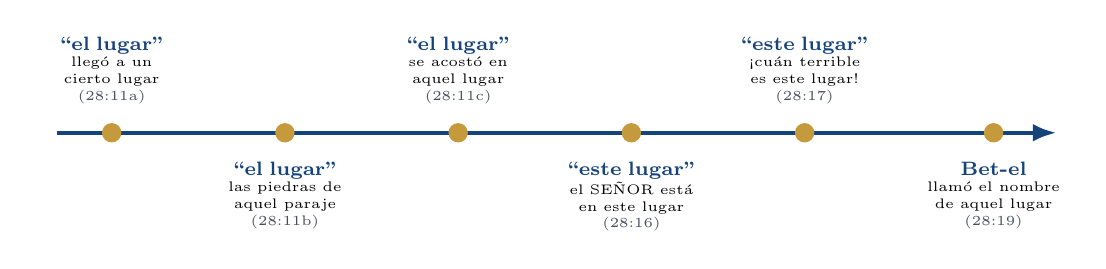
\begin{tikzpicture}[font=\tiny]
 \draw[line width=1.6pt,azul,-{Latex[length=3mm]}] (-0.3,0) -- (12.4,0);
 \foreach \x/\t/\b/\r/\pos in {0.4/{``el lugar''}/{llegó a un cierto lugar}/{28:11a}/above,
   2.6/{``el lugar''}/{las piedras de aquel paraje}/{28:11b}/below,
   4.8/{``el lugar''}/{se acostó en aquel lugar}/{28:11c}/above,
   7.0/{``este lugar''}/{el \SENOR{} está en este lugar}/{28:16}/below,
   9.2/{``este lugar''}/{¡cuán terrible es este lugar!}/{28:17}/above,
   11.6/{Bet-el}/{llamó el nombre de aquel lugar}/{28:19}/below}{
  \fill[dorado] (\x,0) circle (3.5pt);
  \node[\pos=7pt,text width=1.9cm,align=center] at (\x,0) {\textbf{\textcolor{azul}{\scriptsize\t}}\\ \b\\ {\color{gris}(\r)}};}
\end{tikzpicture}\par\medskip
\small\RaggedRight \heb{מָקוֹם} seis veces en Gn 28:11--19 (conteo propio en la BHS). El relato pasa de ``un cierto lugar'' a ``este lugar'' donde está el \SENOR{}, y de ahí a un lugar con nombre.
\end{frame}

\begin{frame}{``Y yo no lo sabía''}
\centering
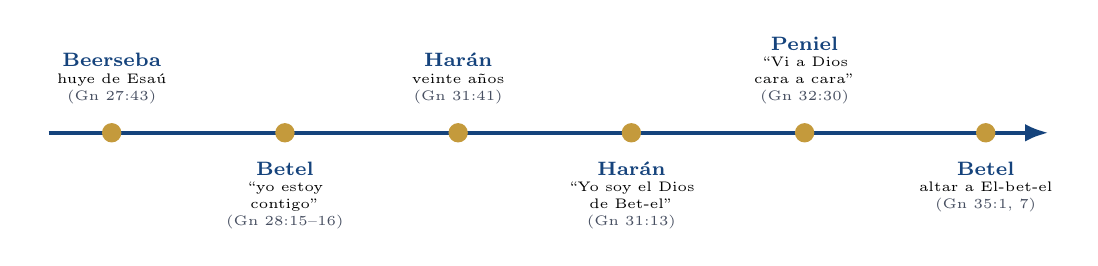
\begin{tikzpicture}[font=\tiny]
 \draw[line width=1.6pt,azul,-{Latex[length=3mm]}] (-0.3,0) -- (12.4,0);
 \foreach \x/\t/\b/\r/\pos in {0.5/{Beerseba}/{huye de Esaú}/{Gn 27:43}/above,
   2.7/{Betel}/{``yo estoy contigo''}/{Gn 28:15--16}/below,
   4.9/{Harán}/{veinte años}/{Gn 31:41}/above,
   7.1/{Harán}/{``Yo soy el Dios de Bet-el''}/{Gn 31:13}/below,
   9.3/{Peniel}/{``Vi a Dios cara a cara''}/{Gn 32:30}/above,
   11.6/{Betel}/{altar a El-bet-el}/{Gn 35:1, 7}/below}{
  \fill[dorado] (\x,0) circle (3.5pt);
  \node[\pos=7pt,text width=1.9cm,align=center] at (\x,0) {\textbf{\textcolor{azul}{\scriptsize\t}}\\ \b\\ {\color{gris}(\r)}};}
\end{tikzpicture}\par\medskip
\begin{columns}[t,onlytextwidth]
\begin{column}{0.52\textwidth}\small
\begin{itemize}
\item Jacob no descubre que Dios está \emph{solo} en Betel, sino que estaba donde él no lo esperaba.
\item El ``Dios de Bet-el'' le habla en Harán (31:13): su nombre recuerda un lugar, pero no está atado a él.
\end{itemize}
\end{column}
\begin{column}{0.46\textwidth}\scriptsize
Henry: ``Doquiera estemos, en la ciudad o en el desierto\ldots{} en la tienda o en la calle, podemos mantener nuestra relación con el Cielo'' (Henry, 1999, Gn 28:16--19).\par\smallskip
\precision{la tradición rabínica lee \heb{וַיִּפְגַּע} como oración (cf. Jer 7:16): Jacob instituyó la oración de la tarde (\emph{Berajot} 26b).}
\end{column}
\end{columns}
\end{frame}

% ------------------------------------------------------------------
\section{Judaísmo}

\begin{frame}{\emph{HaMaqom}: el Lugar del mundo}
\begin{center}\scriptsize\heb{מִפְּנֵי מָה מְכַנִּין שְׁמוֹ שֶׁל הַקָּדוֹשׁ בָּרוּךְ הוּא וְקוֹרְאִין אוֹתוֹ מָקוֹם}\\[1pt]\heb{שֶׁהוּא מְקוֹמוֹ שֶׁל עוֹלָם וְאֵין עוֹלָמוֹ מְקוֹמוֹ}\end{center}
\begin{columns}[t,onlytextwidth]
\begin{column}{0.54\textwidth}\small
``¿Por qué se da al Santo, bendito sea, el sobrenombre de \emph{Maqom}? Porque él es el lugar del mundo, y el mundo no es su lugar'' (\emph{Bereshit Rabá} 68:9, sobre Gn 28:11).
\begin{itemize}
\item Prueba: ``He aquí un lugar junto a mí'' (Éx 33:21).
\item Parábola: el caballo depende del jinete, no el jinete del caballo (Hab 3:8).
\end{itemize}
\end{column}
\begin{column}{0.44\textwidth}\scriptsize
\textbf{En la oración:} ``misericordia y súplica delante de \emph{HaMaqom}'' (\emph{Avot} 2:13).\par\smallskip
\textbf{En el duelo:} \heb{הַמָּקוֹם יְנַחֵם אֶתְכֶם}, ``que \emph{HaMaqom} os consuele\ldots''.\par\smallskip
\precision{interpretación rabínica (Sefaria); traducción propia. La fórmula de duelo es costumbre asquenazí.}
\end{column}
\end{columns}
\end{frame}

\begin{frame}{``No hay lugar vacío de la Shejiná''}
\scriptsize\renewcommand{\arraystretch}{1.18}
\begin{tabular}{@{}>{\RaggedRight\arraybackslash}p{2.3cm}>{\RaggedRight\arraybackslash}p{9.5cm}@{}}
\toprule
\emph{Shemot Rabá} 2:5 & ¿Por qué habló Dios desde una zarza? \heb{שֶׁאֵין מָקוֹם פָּנוּי בְּלֹא שְׁכִינָה אֲפִלּוּ סְנֶה}: ``no hay lugar vacío de la Shejiná, ni siquiera una zarza''. \\
\emph{Bava Batra} 25a & Rabí Oshayá: \heb{שְׁכִינָה בְּכׇל מָקוֹם}, ``la Shejiná está en todo lugar''; prueba: Neh 9:6. \\
\emph{Sanedrín} 39a & ``¿Cuántas Shejinás hay?'', pregunta el emperador. Gamliel: si el sol, un siervo de Dios, alumbra todo el mundo, ``¡cuánto más la Shejiná del Santo!''. \\
\emph{Berajot} 10a & ``Como el Santo, bendito sea, llena todo el mundo, así el alma llena todo el cuerpo''. \\
\bottomrule
\end{tabular}\par\medskip
\begin{columns}[t,onlytextwidth]
\begin{column}{0.52\textwidth}\small
\heb{שְׁכִינָה}, de \heb{שׁכן} ``habitar'': el término rabínico para la presencia que habita. La presencia ``en medio de diez'' no divide a Dios. Jesús: ``donde están dos o tres\ldots{} allí estoy yo'' (Mt 18:20).
\end{column}
\begin{column}{0.46\textwidth}
\precision{interpretaciones rabínicas (Sefaria); traducción propia.}
\end{column}
\end{columns}
\end{frame}

\begin{frame}{La \emph{Qedushá}: ``¿dónde está el lugar de su gloria?''}
\begin{center}\heb{כְּבוֹדוֹ מָלֵא עוֹלָם}\\[2pt]\heb{מְשָׁרְתָיו שׁוֹאֲלִים זֶה לָזֶה אַיֵּה מְקוֹם כְּבוֹדוֹ}\end{center}
\begin{tcolorbox}[colback=papiro,colframe=dorado,boxrule=1.2pt,arc=3pt]
\small ``Su gloria llena el mundo; sus servidores se preguntan unos a otros: ¿Dónde está el lugar de su gloria?'' (\emph{Sidur}, \emph{Qedushá} de \emph{Musaf})
\end{tcolorbox}
\begin{columns}[t,onlytextwidth]
\begin{column}{0.52\textwidth}\small
Entre Is 6:3 (``toda la tierra está llena de su gloria'') y Ez 3:12 (``Bendita sea la gloria de \SENOR{} desde su lugar''), la oración guarda la paradoja.
\end{column}
\begin{column}{0.46\textwidth}\small
Los ángeles saben que la gloria lo llena todo, y por eso no pueden señalar un lugar: el Dios cercano es el Dios lejano.
\end{column}
\end{columns}
\end{frame}

\begin{frame}{Targumes, Maimónides y Qumrán}
\scriptsize\renewcommand{\arraystretch}{1.15}
\begin{tabular}{@{}>{\RaggedRight\arraybackslash}p{2.4cm}>{\RaggedRight\arraybackslash}p{9.4cm}@{}}
\toprule
\textbf{Ónkelos} Gn 28:16 & \heb{בְּקוּשְׁטָא אִית יְקָרָא דַיְיָ שָׁרֵי בְּאַתְרָא הָדֵין}: ``En verdad la \destacar{gloria} del \SENOR{} habita en este lugar''. \\
\textbf{Jonatán} Jer 23:24 & ``¿No llena \destacar{mi gloria} los cielos y la tierra?''. \\
\textbf{Jonatán} Ez 48:35 & ``\ldots haga reposar su \destacar{Shejiná} allí''. \\
\textbf{Maimónides} & \emph{Guía} I:8: \emph{maqom} pasó de ``lugar'' a ``rango''; Ez 3:12 = ``según la excelsitud de su existencia''. I:18: ``cerca'' dicho de Dios es conocimiento, no proximidad física. \\
\textbf{Qumrán} & 11QPs\textsuperscript{a} conserva Sal 139:8--24 (Sanders, 1965): el salmo de la presencia se copiaba y se oraba. \\
\bottomrule
\end{tabular}\par\medskip
\small\RaggedRight Los targumes no niegan la presencia; evitan decir que el ser de Dios ocupe un sitio: hablan de su ``gloria'' o de su ``Shejiná''.\par\smallskip
\precision{lecturas judías antiguas y medievales (Sefaria; Maimónides, 1903); traducción propia. Cotejar 11Q5 en la Leon Levy Dead Sea Scrolls Digital Library.}
\end{frame}

% ------------------------------------------------------------------
\section{En Cristo}

\begin{frame}{Emanuel, de principio a fin}
\begin{columns}[t,onlytextwidth]
\begin{column}{0.50\textwidth}
\begin{cita}[fontupper=\scriptsize\itshape]enseñándoles que guarden todas las cosas que os he mandado; y he aquí yo estoy con vosotros todos los días, hasta el fin del mundo. Amén.\fuente{(Mt 28:20, RVR1960)}\end{cita}
\begin{cita}[fontupper=\scriptsize\itshape]Y aquel Verbo fue hecho carne, y habitó entre nosotros\ldots\fuente{(Jn 1:14, RVR1960)}\end{cita}
\end{column}
\begin{column}{0.48\textwidth}\small
\begin{itemize}
\item \grc{μεθ’ ἡμῶν ὁ θεός} (Mt 1:23) y \grc{ἐγὼ μεθ’ ὑμῶν εἰμι} (28:20): el mismo ``con'' abre y cierra el evangelio.
\item Solo puede prometer estar con todos, todos los días, quien es Dios.
\item \grc{ἐσκήνωσεν}: ``puso su tienda'', el lenguaje del tabernáculo.
\end{itemize}
\precision{la correspondencia 1:23 / 28:20 es una observación literaria de muchos intérpretes.}
\end{column}
\end{columns}
\end{frame}

\begin{frame}{Betel en Juan 1:51}
\scriptsize\renewcommand{\arraystretch}{1.18}
\begin{tabular}{@{}>{\RaggedRight\arraybackslash}p{1.6cm}>{\RaggedRight\arraybackslash}p{5.0cm}>{\RaggedRight\arraybackslash}p{5.2cm}@{}}
\toprule
 & \textbf{Gn 28:12 (LXX)} & \textbf{Jn 1:51} \\ \midrule
Ángeles & \grc{οἱ ἄγγελοι τοῦ θεοῦ ἀνέβαινον καὶ κατέβαινον} & \grc{τοὺς ἀγγέλους τοῦ θεοῦ ἀναβαίνοντας καὶ καταβαίνοντας} \\
Sobre & \grc{ἐπ’ αὐτῆς}, ``sobre ella'' (la escalera) & \grc{ἐπὶ τὸν υἱὸν τοῦ ἀνθρώπου}, ``sobre el Hijo del Hombre'' \\
Lugar & ``casa de Dios, y puerta del cielo'' (28:17) & ``veréis el cielo abierto'' \\
\bottomrule
\end{tabular}\par\medskip
\begin{columns}[t,onlytextwidth]
\begin{column}{0.52\textwidth}
\begin{cita}[fontupper=\scriptsize\itshape]De aquí adelante veréis el cielo abierto, y a los ángeles de Dios que suben y descienden sobre el Hijo del Hombre.\fuente{(Jn 1:51, RVR1960)}\end{cita}
\end{column}
\begin{column}{0.46\textwidth}\small
La escalera de Jacob es ahora una persona. El lugar donde el cielo toca la tierra ya no es Betel: es \destacar{Jesús}. ``Mas él hablaba del templo de su cuerpo'' (Jn 2:21).
\end{column}
\end{columns}
\end{frame}

\begin{frame}{Pablo en Atenas}
\begin{columns}[t,onlytextwidth]
\begin{column}{0.52\textwidth}
\begin{cita}[fontupper=\scriptsize\itshape]El Dios que hizo el mundo y todas las cosas que en él hay, siendo Señor del cielo y de la tierra, no habita en templos hechos por manos humanas\ldots{} aunque ciertamente no está lejos de cada uno de nosotros. Porque en él vivimos, y nos movemos, y somos; como algunos de vuestros propios poetas también han dicho: Porque linaje suyo somos.\fuente{(Hch 17:24, 27--28, RVR1960)}\end{cita}
\end{column}
\begin{column}{0.46\textwidth}\small
\begin{itemize}
\item Primero la inmensidad (no en templos), después la cercanía: \grc{οὐ μακρὰν ἀπὸ ἑνὸς ἑκάστου ἡμῶν}.
\item \grc{ἐν αὐτῷ γὰρ ζῶμεν καὶ κινούμεθα καὶ ἐσμέν}: vida, actividad, existencia.
\item No para decir que todos ya están en comunión, sino para llamar al arrepentimiento ``en todo lugar'' (17:30).
\end{itemize}
\end{column}
\end{columns}\par\smallskip
\precision{``linaje suyo somos'': Arato, \emph{Fenómenos} 5; ``en él vivimos'' se atribuye a Epiménides (MacArthur, 2011), atribución discutida (Bruce, 1990). Discurso transmitido por Lucas.}
\end{frame}

\begin{frame}{``Para llenarlo todo''}
\fotolado{panel_efesios4.jpg}{Elaboración propia: Ef 4:10 en escritura uncial (texto NA28).}
\begin{columns}[c,onlytextwidth]
\begin{column}{0.58\textwidth}
\begin{cita}[fontupper=\scriptsize\itshape]la cual es su cuerpo, la plenitud de Aquel que todo lo llena en todo.\fuente{(Ef 1:23, RVR1960)}\end{cita}
\begin{cita}[fontupper=\scriptsize\itshape]Y eso de que subió, ¿qué es, sino que también había descendido primero a las partes más bajas de la tierra? El que descendió, es el mismo que también subió por encima de todos los cielos para llenarlo todo.\fuente{(Ef 4:9--10, RVR1960)}\end{cita}
\end{column}
\begin{column}{0.40\textwidth}\end{column}
\end{columns}
\end{frame}

\begin{frame}{De Jeremías a Efesios}
\scriptsize\renewcommand{\arraystretch}{1.2}
\begin{tabular}{@{}>{\RaggedRight\arraybackslash}p{1.9cm}>{\RaggedRight\arraybackslash}p{6.0cm}>{\RaggedRight\arraybackslash}p{3.9cm}@{}}
\toprule
\textbf{Texto} & \textbf{Griego} & \textbf{Sujeto} \\ \midrule
Jer 23:24 LXX & \grc{μὴ οὐχὶ τὸν οὐρανὸν καὶ τὴν γῆν ἐγὼ πληρῶ;} & el \SENOR \\
Ef 1:23 & \grc{τὸ πλήρωμα τοῦ τὰ πάντα ἐν πᾶσιν πληρουμένου} & Cristo, cabeza \\
Ef 4:10 & \grc{ἵνα πληρώσῃ τὰ πάντα} & Cristo, que descendió y subió \\
\bottomrule
\end{tabular}\par\medskip
\begin{columns}[t,onlytextwidth]
\begin{column}{0.52\textwidth}\small
\begin{itemize}
\item Lo que en Jeremías es prerrogativa del \SENOR, en Efesios es obra de Cristo exaltado.
\item Descendió a lo más bajo y subió sobre todos los cielos: los extremos del Salmo 139.
\end{itemize}
\end{column}
\begin{column}{0.46\textwidth}
\precision{autoría de Efesios discutida; \grc{πληρουμένου} puede ser media (``que llena'') o pasiva (Lincoln, 1990). En carta indiscutida: ``un Señor, Jesucristo, por medio del cual son todas las cosas'' (1 Co 8:6).}
\end{column}
\end{columns}
\end{frame}

\begin{frame}{``Cerca de ti está la palabra''}
\scriptsize\renewcommand{\arraystretch}{1.18}
\begin{tabular}{@{}>{\RaggedRight\arraybackslash}p{3.9cm}>{\RaggedRight\arraybackslash}p{3.7cm}>{\RaggedRight\arraybackslash}p{4.2cm}@{}}
\toprule
\textbf{Dt 30:12--14} & \textbf{Ro 10:6--8} & \textbf{Lectura de Pablo} \\ \midrule
``¿Quién subirá por nosotros al cielo?'' & ``¿Quién subirá al cielo?'' & ``para traer abajo a Cristo'' \\
``¿Quién pasará por nosotros el mar?'' & ``¿quién descenderá al abismo?'' & ``para hacer subir a Cristo de entre los muertos'' \\
``muy cerca de ti está la palabra'' & ``Cerca de ti está la palabra'' & ``la palabra de fe que predicamos'' \\
\bottomrule
\end{tabular}\par\medskip
\begin{columns}[t,onlytextwidth]
\begin{column}{0.52\textwidth}\small
No hace falta subir al cielo ni bajar al abismo para encontrar a Dios: Cristo ya bajó y ya subió. \grc{ἐγγύς σου τὸ ῥῆμά ἐστιν}. Hays (1989) estudia el pasaje como ejemplo de la relectura paulina de la Escritura.
\end{column}
\begin{column}{0.46\textwidth}
\precision{Pablo cambia ``el mar'' por ``el abismo'' (cf. Sal 107:26). El eco del Sal 139:8 (cielos y Seol) es posible, no explícito.}
\end{column}
\end{columns}
\end{frame}

\begin{frame}{Ni lo alto ni lo profundo}
\begin{columns}[c,onlytextwidth]
\begin{column}{0.52\textwidth}
\begin{cita}[fontupper=\scriptsize\itshape]Por lo cual estoy seguro de que ni la muerte, ni la vida, ni ángeles, ni principados, ni potestades, ni lo presente, ni lo por venir, ni lo alto, ni lo profundo, ni ninguna otra cosa creada nos podrá separar del amor de Dios, que es en Cristo Jesús Señor nuestro.\fuente{(Ro 8:38--39, RVR1960)}\end{cita}
\end{column}
\begin{column}{0.46\textwidth}\small
\begin{itemize}
\item \grc{οὔτε ὕψωμα οὔτε βάθος}: todo el espacio creado.
\item El salmista no hallaba dónde huir de Dios; Pablo no halla dónde el amor de Dios en Cristo no alcance.
\item La omnipresencia, vista desde la cruz, es \destacar{seguridad}.
\end{itemize}
\precision{posibles términos astrológicos (Moo, 1996); la relación con el Sal 139 es un posible eco.}
\end{column}
\end{columns}
\end{frame}

\begin{frame}{El templo que es un pueblo}
\begin{columns}[t,onlytextwidth]
\begin{column}{0.50\textwidth}
\begin{cita}[fontupper=\scriptsize\itshape]¿No sabéis que sois templo de Dios, y que el Espíritu de Dios mora en vosotros?\fuente{(1 Co 3:16, RVR1960)}\end{cita}
\begin{cita}[fontupper=\scriptsize\itshape]Porque vosotros sois el templo del Dios viviente, como Dios dijo: Habitaré y andaré entre ellos, Y seré su Dios, Y ellos serán mi pueblo.\fuente{(2 Co 6:16b, RVR1960)}\end{cita}
\end{column}
\begin{column}{0.48\textwidth}\small
\begin{itemize}
\item Pablo cita Lv 26:11--12 y Ez 37:27: \grc{ἐνοικήσω ἐν αὐτοῖς καὶ ἐμπεριπατήσω}.
\item El Dios que llena el cielo y la tierra habita en un pueblo de judíos y gentiles, ``morada de Dios en el Espíritu'' (Ef 2:22).
\item Es el cumplimiento de \SENOR-sama: Dios está allí, en medio de los suyos.
\end{itemize}
\end{column}
\end{columns}
\end{frame}

\begin{frame}{``El Señor está cerca''}
\begin{columns}[c,onlytextwidth]
\begin{column}{0.50\textwidth}
\begin{cita}Vuestra gentileza sea conocida de todos los hombres. El Señor está cerca. Por nada estéis afanosos, sino sean conocidas vuestras peticiones delante de Dios en toda oración y ruego, con acción de gracias.\fuente{(Flp 4:5--6, RVR1960)}\end{cita}
\end{column}
\begin{column}{0.48\textwidth}\small
\begin{itemize}
\item \grc{ὁ κύριος ἐγγύς} reproduce el \grc{ἐγγὺς κύριος} del Sal 144:18 LXX [145:18].
\item La cercanía del Señor es la razón para \destacar{orar} en lugar de angustiarse.
\end{itemize}
\precision{sentido temporal (la venida está próxima) o espacial (el Señor presente); Fee (1995) ve el eco del Sal 145:18 y no excluye el temporal.}
\end{column}
\end{columns}
\end{frame}

\begin{frame}{Cristo y la omnipresencia}
\begin{columns}[t,onlytextwidth]
\begin{column}{0.50\textwidth}\small
¿Cómo puede un hombre resucitado estar ``con vosotros todos los días''?
\begin{itemize}
\item \textbf{Calvino (1960)}: según su divinidad, el Hijo llena el mundo; su humanidad glorificada está en un lugar.
\end{itemize}
\end{column}
\begin{column}{0.48\textwidth}
\begin{tcolorbox}[colback=papiro,colframe=dorado,boxrule=1.2pt,arc=3pt]
\scriptsize ``El Hijo de Dios descendió del cielo de tal modo que, sin dejar el cielo, quiso nacer en el vientre de la virgen, andar por la tierra y ser colgado en la cruz; y sin embargo llenaba continuamente el mundo, como lo había hecho desde el principio'' (Calvino, 1960, II, 13, 4).
\end{tcolorbox}
\precision{traducción propia.}
\end{column}
\end{columns}
\end{frame}

\begin{frame}{La presencia de Dios, revelada en Cristo}
\centering
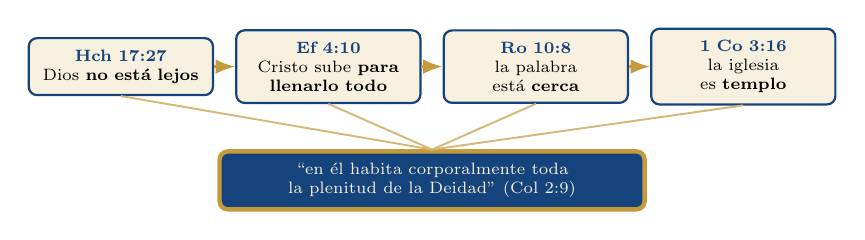
\begin{tikzpicture}[font=\scriptsize,scale=0.85,transform shape]
 \foreach \x/\n/\t/\d in {0/a/{Hch 17:27}/{Dios \textbf{no está lejos}},
   3.1/b/{Ef 4:10}/{Cristo sube \textbf{para llenarlo todo}},
   6.2/c/{Ro 10:8}/{la palabra está \textbf{cerca}},
   9.3/d/{1 Co 3:16}/{la iglesia es \textbf{templo}}}{
  \node[caja,text width=2.4cm,align=center] (\n) at (\x,0) {\textbf{\textcolor{azul}{\t}}\\ \d};}
 \draw[-{Latex[length=2.5mm]},dorado,line width=1.1pt](a)--(b); \draw[-{Latex[length=2.5mm]},dorado,line width=1.1pt](b)--(c); \draw[-{Latex[length=2.5mm]},dorado,line width=1.1pt](c)--(d);
 \node[draw=dorado,line width=1.6pt,fill=azul,text=papiro,rounded corners=3pt,text width=6.0cm,align=center,inner sep=5pt] (e) at (4.65,-1.7) {``en él habita corporalmente toda la plenitud de la Deidad'' (Col 2:9)};
 \foreach \i in {a,b,c,d}\draw[dorado!70,line width=0.7pt](\i.south)--(e.north);
\end{tikzpicture}\par\medskip
\small\RaggedRight Pablo sigue confesando que Dios llena el cielo y la tierra, pero ahora sabe dónde se deja encontrar: en Cristo, en la palabra predicada y en el pueblo donde habita por su Espíritu. \SENOR-sama tiene nombre propio: \destacar{Emanuel}.
\end{frame}

% ------------------------------------------------------------------
\section{Vivirlo}

\begin{frame}{No hay dónde huir}
\begin{columns}[t,onlytextwidth]
\begin{column}{0.50\textwidth}
\begin{cita}[fontupper=\scriptsize\itshape]Y Jonás se levantó para huir de la presencia de \SENOR{} a Tarsis, y descendió a Jope\ldots\fuente{(Jon 1:3, RVR1960)}\end{cita}
\begin{cita}[fontupper=\scriptsize\itshape]Invoqué en mi angustia a \SENOR, y él me oyó; Desde el seno del Seol clamé, Y mi voz oíste.\fuente{(Jon 2:2 [2:3], RVR1960)}\end{cita}
\end{column}
\begin{column}{0.48\textwidth}\small
\begin{itemize}
\item Jonás intentó lo que el Sal 139 declara imposible: \heb{לִבְרֹחַ}, ``huir''.
\item Bajó a Jope, a la nave, al fondo del barco (\heb{יָרַד}), al mar.
\item Desde lo más bajo oró, y fue oído. Huir de Dios es imposible; \destacar{volver} a él siempre es posible.
\end{itemize}
\end{column}
\end{columns}
\end{frame}

\begin{frame}{Delante de Dios, en todo lugar}
\scriptsize\renewcommand{\arraystretch}{1.2}
\begin{tabular}{@{}>{\RaggedRight\arraybackslash}p{2.6cm}>{\RaggedRight\arraybackslash}p{9.2cm}@{}}
\toprule
No hay pecado oculto & ``Los ojos de \SENOR{} están en todo lugar'' (Pr 15:3). José, sin testigos: ``¿cómo, pues, haría yo este grande mal, y pecaría contra Dios?'' (Gn 39:9). \\
No hay soledad & ``Cuando pases por las aguas, yo estaré contigo'' (Is 43:2); ``No te desampararé, ni te dejaré'' (He 13:5; Dt 31:6). \\
No hay lugar sin oración & ``ora a tu Padre que está en secreto'' (Mt 6:6); ``que los hombres oren en todo lugar'' (1 Ti 2:8). Un hospital, una cocina, un bus pueden ser Betel. \\
No hay rincón sin misión & ``id, y haced discípulos a todas las naciones\ldots{} y he aquí yo estoy con vosotros'' (Mt 28:19--20). \\
\bottomrule
\end{tabular}\par\medskip
\small\RaggedRight La presencia de Dios no quita el valle, pero cambia al que camina por él: ``Aunque ande en valle de sombra de muerte, no temeré mal alguno, porque tú estarás conmigo'' (Sal 23:4).
\end{frame}

\begin{frame}{Cinco respuestas al Dios presente}
\centering
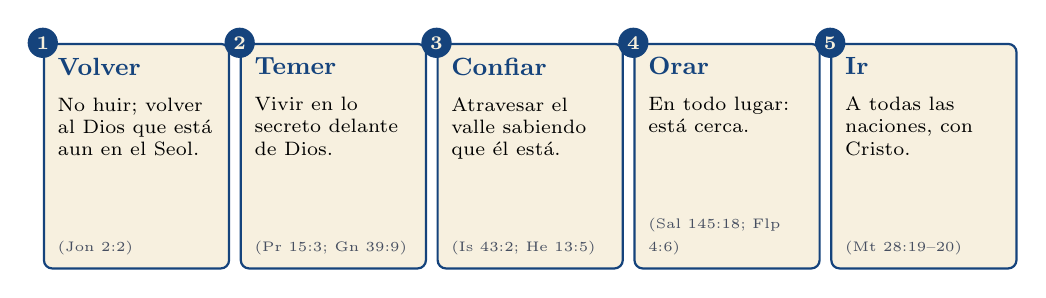
\begin{tikzpicture}
 \foreach \x/\n/\t/\d/\r in {0/1/{Volver}/{No huir; volver al Dios que está aun en el Seol.}/{Jon 2:2},
   2.5/2/{Temer}/{Vivir en lo secreto delante de Dios.}/{Pr 15:3; Gn 39:9},
   5.0/3/{Confiar}/{Atravesar el valle sabiendo que él está.}/{Is 43:2; He 13:5},
   7.5/4/{Orar}/{En todo lugar: está cerca.}/{Sal 145:18; Flp 4:6},
   10.0/5/{Ir}/{A todas las naciones, con Cristo.}/{Mt 28:19--20}}{
  \node[caja,anchor=north] (b\n) at (\x,0) {\parbox[t][2.5cm][t]{2.0cm}{\RaggedRight
    {\small\textbf{\textcolor{azul}{\t}}}\\[5pt]\scriptsize \d\par\vfill{\tiny\color{gris}(\r)}}};
  \node[circle,fill=azul,text=papiro,font=\scriptsize\bfseries,inner sep=1.6pt] at (b\n.north west) {\n};}
\end{tikzpicture}\par\medskip
\small\RaggedRight ``En tu presencia hay plenitud de gozo; delicias a tu diestra para siempre'' (Sal 16:11).
\end{frame}

% ------------------------------------------------------------------
\section{Síntesis}

\begin{frame}{Síntesis}
\begin{tcolorbox}[colback=papiro,colframe=azul,boxrule=1pt,arc=3pt]
\scriptsize ``¿No lleno yo, dice \SENOR, el cielo y la tierra?'' (Jer 23:24). Ningún lugar lo contiene (1 R 8:27) y está en todo lugar con todo su ser. Israel lo dijo con un rostro que acompaña (\emph{panim}), un ``allí'' en cada extremo (\emph{sham}), un ``contigo'' (\emph{im}) y un ``cerca'' (\emph{qarov}). En Betel, Jacob descubrió que ``\SENOR{} está en este lugar, y yo no lo sabía''; el judaísmo llamó a Dios \emph{HaMaqom}. El Nombre es \SENOR-sama (Ez 48:35), y su cumplimiento, Emanuel. Pablo lo ve en Cristo, que subió ``para llenarlo todo'' (Ef 4:10), en la palabra cercana (Ro 10:8) y en la iglesia, templo del Dios viviente (2 Co 6:16).
\end{tcolorbox}
\scriptsize\renewcommand{\arraystretch}{1.12}
\begin{tabular}{@{}>{\RaggedRight\arraybackslash}p{2.0cm}>{\RaggedRight\arraybackslash}p{9.8cm}@{}}
\toprule
\textbf{Mirada} & \textbf{Aporte} \\ \midrule
Hebrea & tres preguntas (Jer 23:23--24); \emph{panim, sham, im, qarov, maqom, male', kul}; \SENOR-sama; Betel. \\
Judía & \emph{HaMaqom} (Bereshit Rabá 68:9); ninguna zarza sin Shejiná; la \emph{Qedushá}; los targumes; Maimónides; Qumrán. \\
Teológica & omnipresente porque es Espíritu (Jn 4:24); inmenso (1 R 8:27); Rey en todo lugar (Is 66:1); presencia que ve (Pr 15:3); Agustín, Charnock, Berkhof, Washer. \\
Paulina & no lejos (Hch 17:27); todo lo llena (Ef 4:10); cerca la palabra (Ro 10:8); templo (1 Co 3:16); ``el Señor está cerca'' (Flp 4:5). \\
\bottomrule
\end{tabular}
\end{frame}

\begin{frame}{Para la reflexión}
\begin{cita}Mas alábese en esto el que se hubiere de alabar: en entenderme y conocerme, que yo soy \SENOR, que hago misericordia, juicio y justicia en la tierra; porque estas cosas quiero, dice \SENOR.\fuente{(Jer 9:24 [9:23], RVR1960)}\end{cita}
\small
\begin{itemize}
\item ¿Hay algún ``Tarsis'' al que intento huir de la presencia de Dios?
\item ¿Qué cambiaría en lo que hago a solas si recordara que Dios está allí (Pr 15:3)?
\item ¿En qué ``cierto lugar'' de mi vida Dios estaba, y yo no lo sabía (Gn 28:16)?
\item ¿Oro solo en ciertos lugares, o en todo lugar, porque el Señor está cerca (Flp 4:5--6)?
\end{itemize}
\end{frame}

% ------------------------------------------------------------------
\section{Glosario}

\begin{frame}{Glosario}
\scriptsize
\begin{columns}[t,onlytextwidth]
\begin{column}{0.49\textwidth}
\begin{description}\setlength{\itemsep}{1pt}
\item[\emph{Coram Deo}] (latín) ``delante de Dios''.
\item[\emph{Engýs}] (\grc{ἐγγύς}) cerca (Ro 10:8; Flp 4:5).
\item[\emph{HaMaqom}] (\heb{הַמָּקוֹם}) ``el Lugar'': nombre rabínico de Dios.
\item[\emph{Im}] (\heb{עִם}) con (Gn 28:15; Is 7:14).
\item[Inmensidad] ningún espacio contiene a Dios (1 R 8:27).
\item[\emph{Kul}] (\heb{כּוּל}) contener (1 R 8:27).
\item[\emph{Male'}] (\heb{מָלֵא}) llenar (Is 6:3; Jer 23:24).
\item[\emph{Maqom}] (\heb{מָקוֹם}) lugar (Gn 28:11--19).
\end{description}
\end{column}
\begin{column}{0.49\textwidth}
\begin{description}\setlength{\itemsep}{1pt}
\item[Omnipresencia] Dios presente con todo su ser en todo lugar.
\item[\emph{Panim}] (\heb{פָּנִים}) rostro, presencia (Éx 33:14).
\item[\emph{Páreimi}] (\grc{πάρειμι}) estar presente (Sal 138:8 LXX).
\item[\emph{Plēróō}] (\grc{πληρόω}) llenar (Ef 4:10).
\item[\emph{Qarov}] (\heb{קָרוֹב}) cercano (Sal 145:18).
\item[\emph{Sham}] (\heb{שָׁם}) allí (Sal 139:8; Ez 48:35).
\item[Shejiná] (\heb{שְׁכִינָה}) presencia que habita (rabínico).
\item[\emph{Sullam}] (\heb{סֻלָּם}) escalera (Gn 28:12).
\end{description}
\end{column}
\end{columns}
\end{frame}

% ------------------------------------------------------------------
\section{Referencias}

\begin{frame}{Referencias}
\fontsize{5.1}{6.1}\selectfont
\begin{columns}[t,onlytextwidth]
\begin{column}{0.49\textwidth}
\refapa{Agustín de Hipona. (s.f.). \emph{Confesiones} [I, 3, 3]. (Obra original escrita ca. 397--400)}
\refapa{Berkhof, L. (1938). \emph{Systematic theology}. Eerdmans.}
\refapa{Bruce, F.~F. (1990). \emph{The Acts of the Apostles: The Greek text with introduction and commentary} (3.ª ed.). Eerdmans.}
\refapa{Calvino, J. (1960). \emph{Institutes of the Christian religion} (J.~T. McNeill, Ed.; F.~L. Battles, Trad.). Westminster Press. (Obra original publicada en 1559)}
\refapa{Elliger, K., \& Rudolph, W. (Eds.). (1997). \emph{Biblia Hebraica Stuttgartensia} (5.ª ed.). Deutsche Bibelgesellschaft.}
\refapa{Fee, G.~D. (1995). \emph{Paul's letter to the Philippians}. Eerdmans.}
\refapa{Hays, R.~B. (1989). \emph{Echoes of Scripture in the letters of Paul}. Yale University Press.}
\refapa{Henry, M. (1999). \emph{Comentario bíblico de Matthew Henry} (F. Lacueva, Trad.). Editorial CLIE.}
\refapa{Lincoln, A.~T. (1990). \emph{Ephesians} (WBC 42). Word Books.}
\refapa{MacArthur, J. (2011). \emph{Biblia de estudio MacArthur} (notas). Grupo Nelson.}
\refapa{Maimónides. (1903). \emph{The guide for the perplexed} (M. Friedländer, Trad.; 2.ª ed.) [I, 8; I, 18]. Sefaria. https://www.sefaria.org}
\refapa{\emph{Midrash Rabá}: \emph{Bereshit Rabá} [68:9]; \emph{Shemot Rabá} [2:5]. (s.f.). Sefaria. https://www.sefaria.org}
\refapa{\emph{Misná: Pirké Avot} [2:13]. (s.f.). Sefaria. https://www.sefaria.org}
\end{column}
\begin{column}{0.49\textwidth}
\refapa{Moo, D.~J. (1996). \emph{The epistle to the Romans}. Eerdmans.}
\refapa{Nestle, E., \& Aland, K. (Eds.). (2012). \emph{Novum Testamentum Graece} (28.ª ed.). Deutsche Bibelgesellschaft.}
\refapa{Pink, A.~W. (2020). \emph{Los atributos de Dios} (E. Rodríguez Cruz, Trad.). Chapel Library. (Obra original publicada en 1930)}
\refapa{Rahlfs, A., \& Hanhart, R. (Eds.). (2006). \emph{Septuaginta} (Ed. rev.). Deutsche Bibelgesellschaft.}
\refapa{Sanders, J.~A. (1965). \emph{The Psalms scroll of Qumrân Cave 11 (11QPs\textsuperscript{a})} (DJD IV). Clarendon Press.}
\refapa{\emph{Santa Biblia: Reina-Valera 1960}. (1960). Sociedades Bíblicas en América Latina.}
\refapa{\emph{Sidur asquenazí} [\emph{Qedushá} de \emph{Musaf}]. (s.f.). Sefaria. https://www.sefaria.org}
\refapa{Steinsaltz, A. (Ed.). (2017). \emph{Koren Talmud Bavli: Edición William Davidson} [Bava Batra 25a; Berajot 10a, 26b; Sanedrín 39a]. Sefaria. https://www.sefaria.org}
\refapa{\emph{Targum Ónkelos} [Gn 28:16]; \emph{Targum Jonatán a los Profetas} [Jer 23:23--24; Ez 48:35]. (s.f.). Sefaria. https://www.sefaria.org}
\refapa{Vine, W.~E. (1999). \emph{Diccionario expositivo de palabras del Antiguo y del Nuevo Testamento exhaustivo}. Caribe.}
\refapa{Washer, P.~D. (2021). \emph{Conociendo al Dios vivo} (A. Ávila, A. Valverde y J. Namnún, Trads.). Editorial Legado Bautista Confesional; HeartCry. (Obra original publicada en 2016)}
\end{column}
\end{columns}
\par\smallskip{\color{gris}Las citas bíblicas son de la Reina-Valera 1960; ``Jehová'' se reemplaza por \SENOR. Hebreo: BHS; griego: NA28 y LXX de Rahlfs-Hanhart. Fuentes judías: Sefaria; lo rabínico se marca como \emph{precisión}.}
\end{frame}

\end{document}
